\documentclass{beamer}
%
% Choose how your presentation looks.
%
% For more themes, color themes and font themes, see:
% http://deic.uab.es/~iblanes/beamer_gallery/index_by_theme.html
%
\mode<presentation>
{
  \usetheme{default}      % or try Darmstadt, Madrid, Warsaw, ...
  \usecolortheme{seahorse} % or try albatross, beaver, crane, ...
  \usefonttheme{default}  % or try serif, structurebold, ...
  \setbeamertemplate{navigation symbols}{}
  \setbeamertemplate{caption}[numbered]
} 

\setbeamertemplate{footline}[frame number]
\usepackage[english]{babel}
\usepackage[utf8x]{inputenc}

\title[Intergenerational mobility]{Intergenerational Transfers and Education Policy}
\author{Mariella Gonzales, Rebecca Gorges, Justin Holz, Yuvraj Pathak, Derek Wu}
\institute{ECON 350: Human Capital, Markets, and the Family}
\date{March 8, 2017}

\AtBeginSection[]
{
  \begin{frame}
    \frametitle{Contents}
    \tableofcontents[currentsection, currentsubsection]
  \end{frame}
}

\AtBeginSubsection[]
{
  \begin{frame}
    \frametitle{Contents}
    \tableofcontents[currentsection, currentsubsection]
  \end{frame}
}
\begin{document}


\begin{frame}
\titlepage % Print the title page as the first slide
\end{frame}

\begin{frame}
\frametitle{Contents} % Table of contents slide, comment this block out to remove it
\tableofcontents % Throughout your presentation, if you choose to use \section{} and \subsection{} commands, these will automatically be printed on this slide as an overview of your presentation
\end{frame}

% Uncomment these lines for an automatically generated outline.
%\begin{frame}{Outline}
%  \tableofcontents
%\end{frame}


%------------------------------------------------
%\section{Becker and Tomes} 
%------------------------------------------------

\section{Introduction and Literature Review}

\begin{frame}{Theoretical Basis - Becker and Tomes}

\begin{block}{From Becker Tomes (1986)}An analysis that is adequate to cope with the many aspects of the rise and fall of families must incorporate \textbf{concern by parents for children as expressed in altruism toward children, investments in the human capital of children, assortative mating in marriage markets, the demand for children, the treatment by parents of exceptionally able or handicapped children, and expectations about events in the next or in even later generations}. Although these and other aspects of behavior are incorporated into a consistent framework based on maximizing behavior, we do not pretend to handle them all in a satisfactory manner. However, our approach indicates how a more complete analysis can be developed in the future.
\end{block}
\end{frame}


\begin{frame}
\frametitle{Becker and Tomes 1986}
Model of transmission of earnings, assets and consumption from parents to children 

\begin{itemize}
\item Basic Idea: What are the determinants of intergenerational mobility:
\begin{itemize}
\item Do children of rich (poor) parents tend to be worse (better) off than their parents? 
\end{itemize}

\item Framework for studying intergenerational mobility by considering the following:
\begin{itemize}
\item Altruism of parents 
\item Investment in human capital
\item Credit constraints

\end{itemize}
\end{itemize}
\end{frame}

%.............................................................

\begin{frame}
\frametitle{Becker and Tomes 1986}

\begin{itemize}

\item Endowments are transmitted by a stochastic-linear process:

\begin{align*}
E^i_{t} = \alpha_{t} + h E^i_{t-1} + \nu^i_{t} \\
\text{where h is the degree of $''$inheritability$''$} 
\end{align*}

\item h $<$ 1 $\Rightarrow$  Endowments regress to the mean

\item Assuming that parents know $\nu_{t}$ prior to making investment in children $\Rightarrow$ rate of return on investment is known to parents 

\item $\Rightarrow$ if there are no credit constraints then, rate of return, $r_{m}$, will be equal to interest rate $r_{t}$ 
\end{itemize}
\end{frame}

%.............................................................

\begin{frame}
\frametitle{Becker and Tomes 1986}

\begin{itemize}
\item Earnings are related directly to human capital, H, by: \\
\begin{center}
Y = H + luck \\
\end{center}

\begin{itemize}
%\begin{align*}
\item where human capital, H, depends on endowments, E; inheritability, h;  and expenditure on development by parents, $x_{t}$ and government, $s_{t}$ 
%\end{align*}
\end{itemize}

\item Dynamic complementarity between endowments and expenditure
\item Marginal return on expenditure, $r_{m}$, decreasing in stock of H

%\item Hence, parents decide between investment in human capital and non-human capital / assets
\item Under no credit constraints, earnings of children only depend on parents' earnings through endowments and its $''$inheritability$''$

\end{itemize}
\end{frame}

%.............................................................

\begin{frame}
\frametitle{Becker and Tomes 1986}

Under credit constraints:  \\
\begin{itemize}
\item Assume investment in human capital of children come at the cost of selling assets, reducing consumption, or increasing labor force activities

\item Cost of expenditure on children now depend directly on parent's earnings in addition to indirect effect through endowments and inheritability 
\begin{align*}
\uparrow \text{expenditure}  \Rightarrow \downarrow \text{ consumption } \Rightarrow  \\
 \uparrow \text{shadow cost of funds (subjective discount rates)} \\
\Rightarrow \text{Smaller cost of investing for higher income parents} 
\end{align*}

\item Effect of endowment on investment is ambiguous
\item Being poor sucks: lower endowment and lower investment
\end{itemize}
\end{frame}

%------------------------------------------------

\begin{frame}
\frametitle{Becker and Tomes 1986}

Non-human capital or assets \\
\begin{itemize}

\item Return on assets assumed to not depend on earnings and endowments
\item Parents will invest in human capital until $r_{m} > r_{t}$, 
\item When $r_{m} \leqq r_{t}$ higher parents' earnings will lead to increase in bequest of assets
\end{itemize}
\end{frame}

%...............................................


%%%%%%%%%%%%%%%%%%%%%%%%%%%%%%%%%%%%%%%%%5
%% Becker Tomes Slides Here
%%%%%%%%%%%%%%%%%%%%%%%%%%%%%%%%%%%%%%%%%5
%\begin{frame}{From Becker and Tomes...}
%\begin{itemize}
%\item Parents display altruism towards children by investing to optimize their potential earnings
%\item But credit constraints affect the schooling decision
%\item Transfer of skills from parents to children
%\end{itemize}
%\end{frame}

\begin{frame}{Becker and Tomes (1986) to Abbott et al (2016) }
\begin{itemize}
\item Quick summary of Becker and Tomes (1986)
\begin{itemize}
\item Inheritability of skills matters for H
\item Altruism on the behalf of utility maximizing parents leads to investment in H
\item Role of credit constraints is important
\end{itemize}

\item From Becker and Tomes (1986) to Abbott et al  (2016)
\begin{itemize}
\item Heterogeneity 
\item Accounts for both altruism and paternalism
\item Explicit treatment of psychic costs - role of cognitive and non-cognitive skills
\item Assortative matching on education 
\end{itemize}
%\item But credit constraints affect the schooling decision
%\item Transfer of skills from parents to children
%\item Psychic costs of schooling also influence the schooling decision
%\item Large portion of labor market outcomes determined by the time the schooling decision is made (eg. Keane and Wolpin)
%\item Transfer of skills from parents to children
%\item Parents display paternalism as well as (or perhaps instead of) altruism
\end{itemize} 
\end{frame}


\begin{frame}{Abbott et al. Introduction}
Abbott, Brant, Giovanni Gallipoli, Costas Meghir, and Giovanni Violante. (2016). "Education Policy and Intergenerational Transfers in Equilibrium," Under revision, Journal of Political Economy. \\

\begin{itemize}
\item Estimate an intergenerational lifecycle general equilibrium human capital investment model 
\item Conduct policy experiments using the model to study the welfare impact of financial aid policies
\end{itemize}
\end{frame}




%%%%%%%%%%%%%%%%%%%%%%%%%%%%%%%%%%%%%%%%%
%%%%%%%%%%%%%%%%%%%%%%%%%%%%%%%%%%%%%%%%%

%\section{Motivation}
%\begin{frame}{Abbott et al. Introduction}
%The model incorporates the following that we've discussed in class:\begin{itemize}
%\item Credit constraints
%\item Matching models for marriage
%\item College decision based on both value and psychic costs
%\item Monetary transfers from parents to children due to altruism and paternalism
%\item Transfers of cognitive and non-cognitive skills from parents to children
%\item Labor supply decisions during and after college
%\item Retirement period(s)
%\end{itemize}
%\end{frame}

\begin{frame}
\frametitle{Abbott et al. Introduction}
Life cycle model of heterogeneous agents facing incomplete financial markets and credit constraints
\begin{itemize}
\item Model earnings by education and gender
\item Allow heterogeneity in returns and costs
\item Explicitly account for psychic costs
\item General equilibrium framework in steady state. In equilibrium:
\begin{itemize}
\item Households choose education, consumption, labor supply, and IVT to maximize expected utility
\item Firms maximize profits
\item All markets clear 
\end{itemize}
\end{itemize}
\end{frame}



\begin{frame}{Abbott et al. Introduction}
Preview of Results
\begin{itemize}
\item Current financial aid system is welfare improving
	\begin{itemize} 
	\item Removal of federal grants and loans would result in reduction of GDP of 4-5\% 
	\end{itemize}
\item Additional loans or grants would not be welfare improving because of crowd out 
	\begin{itemize} 
    \item Additional dollar of government grants would crowd out parental transfers and reduce student's labor supply while in school
	\item However, expansion would benefit small group of high ability, low income, especially girls.
	\end{itemize}
\end{itemize}
\end{frame}


%%%%%%%%%%%%%%%%%%%%%%%%%%%%%%%%%%%%%%%%%%%%%%%%%%%%%%%%%%%%%%%%
%%%%%%%%%%%%%%%%%%%%%%%%%%%%%%%%%%%%%%%%%%%%%%%%%%%%%%%%%%%%%%%%
\section{Model}

\begin{frame}{Timeline of Decisions}
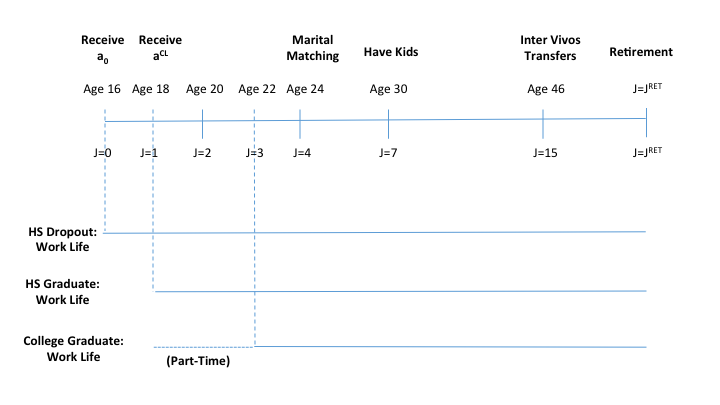
\includegraphics[width=\textwidth]{Timeline.png}
\end{frame}

\begin{frame}{Preferences}
\begin{itemize}
  \item Individual of gender $g$ at age $j$ has the following preferences over consumption $c$ and 				leisure $\ell$:
  		$$u_{gj}(c,\ell) = \frac{c^{1-\gamma}}{1-\gamma} + \vartheta^{g}_{j}\frac{\ell^{1-\nu^{g}_{j}}}			{1-\nu^{g}_{j}},$$
        where $\gamma$ is the coefficient of relative risk aversion, $\nu$ reflects elasticity of labor 		supply, and $\vartheta$ reflects weight placed on $c$ versus $\ell$
  \item Married couples have the following household preferences:
  		$$u_{j}(c^{m},c^{f},\ell^{m},\ell^{f}) = u_{mj}(c^{m},\ell^{m})+u_{fj}(c^{f},							\ell^{f})+x^{m}+x^{f},$$
        where $x^{g}$ denotes utility transfers between spouses, with $x^{m}+x^{f}=0$     
\end{itemize}      
\end{frame}

\begin{frame}{Production}
\begin{itemize}
  \item Representative firm uses physical capital $K$ and human capital $\mathcal{H}$ to produce 				$Y=F(K,\mathcal{H})$, where $F$ is Cobb-Douglas
  \item Aggregate labor input $\mathcal{H}$ is modelled as a CES aggregator of six types of labor 			inputs $H^{e,g}$ indexed by gender $g$ and educational attainment $e\in\left\{LH,HS,CL\right\}$ 		(a la Katz and Murphy, 1992; Heckman et al., 1998)
\end{itemize}      
\end{frame}   

\begin{frame}{Government}
\begin{itemize}
  \item Levies flat taxes $\tau_{w}$, $\tau_{k}$, and $\tau_{c}$ on labor income, asset 						income, and consumption, respectively	
  \item Refunds a lump-sum amount of tax revenue $\varphi$ to each individual (parameterized 		to 			reflect progressive tax system)
  \item Runs a public pension system which pays an education-specific benefit $p^e$ to retirees
  \item Excess tax revenues (net of education and pension systems) spent on non-valued government 				consumption $G$
\end{itemize}      
\end{frame}     

\begin{frame}{Education: Psychic Costs}
\begin{itemize}
  \item Psychic costs (i.e., taste for education) are an important component of schooling decisions (see 		 Cunha et al., 2005; Heckman et al., 2006)
  \item The utility (psychic) cost $\kappa^{e}$ of attaining education level $e$ is linearly 				characterized as:
 		$$\kappa^{e} = \varsigma^{e}_{0}+\varsigma^{e}_{1}\textbf{1}_{\left\{g=f\right							\}}+\varsigma^{e}_{2}\log{(\theta_{non})}+\varsigma^{e}_{3}\log{(\theta_{cog})}+						\varsigma^{e}_{4}\kappa_{\epsilon},$$
        which depends on gender, cognitive skills $\theta_{cog}$, non-cognitive skills 							$\theta_{noncog}$, and an indiosyncratic preference shock $\kappa_{\epsilon}$
  \item Let $\boldsymbol{\theta}=(\theta_{noncog},\theta_{cog})$
\end{itemize}   
\hyperlink{supplemental2}{\beamerbutton{Psychic Cost of Education}}
\end{frame}   

\begin{frame}{Education: High School Continuation Decision (1)}
\begin{itemize}
  \item At $j=0$, this decision is implicitly defined by:
  		\begin{equation*}
  		\begin{aligned}
  		V^*_{g0}(\hat{\textbf{a}},\boldsymbol{\theta},q,\kappa_{\epsilon}) = \mathrm{max}\big\{V_{g0}			(\hat{\textbf{a}},\boldsymbol{\theta},q,\kappa_{\epsilon})-\kappa^{HS}(g,\boldsymbol{\theta},			\kappa_{\epsilon}), \\
        \mathbb{E}_{z}\big[V^{LH}_{g0}(\hat{a}_0,\boldsymbol{\theta},z_0)\big]\big\},
        \end{aligned}
        \end{equation*}
  \item $V^{e}_{gj}(\cdot)$ denotes the value of entering the workforce with education $e$
  \item $V_{gj}(\cdot)$ denotes the value of continuing in school, which includes all costs and 				benefits except for $\kappa^{e}$
  \item Parental wealth classes are indexed by $q=\left\{1,2,3\right\}$, which determines 					qualifications for federal financial aid
\end{itemize}      
\end{frame} 

\begin{frame}{Education: High School Continuation Decision (2)}
\begin{itemize}
  \item Individual who enters labor force at age $j$ with education $e$ solves:
  		$$V^e_{gj}(a_j,\boldsymbol{\theta},z_j) = \underset{c_j,\ell_j,a_{j+1}}{\mathrm{max}}u_g(c_j,			\ell_j)+\beta\mathbb{E}_z\big[V^e_{g,j+1}(a_{j+1},\boldsymbol{\theta},z_{j+1})\big]$$
        subject to
        $$(1+\tau_c)c_j+a_{j+1} = (1-\tau_w)w^{g,e}\varepsilon^{g,e}_j(\boldsymbol{\theta},z_j)					(1-\ell_j)+\varphi+[1+r(1-\tau_k)]a_j,$$
        $$a_{j+1}\geq0,\;c_j\geq0,\;\ell_j\in\big[0,1\big],\;z_{j+1}\sim\Gamma^{g,e}_z(z_{j+1}|z_j).$$        
  \item Here, $a_j$ denotes assets at age $j$, $\varphi$ is the government transfer, $w^{g,e}$ is the 			price for a unit of human capital.
  \item $\varepsilon^{g,e}_j$ is the labor production function and is a function of skills and 					productivity shock $z_j$
\end{itemize}      
\end{frame} 

\begin{frame}{Education: High School Continuation Decision (3)}
\begin{itemize}
  \item The value of completing high school is defined by:
 		$$V_{g0}(\hat{\textbf{a}},\boldsymbol{\theta},q,\kappa_{\epsilon}) = \underset{c_0,a_1}					{\mathrm{max}}\;u_g(c_0,1-\bar{t})+\beta{V}^{*}_{g1}(a_1,\hat{a}^{CL},\boldsymbol{\theta},q,			\kappa_{\epsilon})$$
        subject to
        $$c_0(1+\tau_c) + a_1 = [1+r(1-\tau_k)]\hat{a}_0,$$
        $$a_1\geq0,\;c_0\geq0.$$
  \item High school students are neither permitted to borrow or work and study for a fraction $\bar{t}$ 		of their time endowment
\end{itemize}      
\end{frame} 

\begin{frame}{Education: College Attendance Decision}
\begin{itemize}
  \item The continuation value $V^{*}_{g1}(\cdot)$ is the maximum of the value of attending college and 		the value of entering the labor market as a high school graduate:
    	\begin{equation*}
  		\begin{aligned}
  		V^{*}_{g1}(a_1,\hat{a}^{CL},\boldsymbol{\theta},q,\kappa_{\epsilon}) = \mathrm{max}\big\{V_{g1}			(a_1+\hat{a}^{CL},\boldsymbol{\theta},q)-\kappa^{CL}(g,\boldsymbol{\theta},\kappa_{\epsilon}) \\ 		 \mathbb{E}_{z}\big[V^{HS}_{g1}(\hat{a}_1,\boldsymbol{\theta},z_1)\big]\big\},\big\}
        \end{aligned}
        \end{equation*}
  \item The values of being in college in period $j=1$ and $j=2$ are:      
  		$$V_{g1}(a_1+\hat{a}^{CL},\boldsymbol{\theta},q) = \underset{c_1,\ell_1,a_2,b_2}						{\mathrm{max}}u_g(c_1,\ell_1)+\beta{V}_{g2}(a_2,b_2,\boldsymbol{\theta},q),$$
        $$V_{g2}(a_2,b_2,\boldsymbol{\theta},q) = \underset{c_2,\ell_2,a_3,b_3}{\mathrm{max}}u_g(c_2,			\ell_2)+\beta{V}^{CL}_{g3}(a_3,b_3,\boldsymbol{\theta},q),$$
        where $b_j$ is borrowing at age $j$, $c\geq0$ and $\ell_j\in\big[0,1-\bar{t}\big]$.      
\end{itemize}      
\end{frame} 

\begin{frame}{Education: Budget Constraints (1)}
\begin{center}
  \begin{tabular}{ l | c }
     \hline
     Wealth group & Loan Eligibility \\ \hline
     $q=3$ & Private and Unsubsidized Loans  \\ 
     $q=2$ & Unsubsidized Loans	\\ 
     $q=1$ & Subsidized and Unsubsidized Loans	\\ 
     \hline          
  \end{tabular}
\end{center}
\begin{itemize}
  \item Unsubsidized student loans available up to a limit $\underline{b}$ at an 							interest rate $r^u$  
  \item Subsidized loans available up to a limit $\underline{b}^s$ at no interest
  \item Private loans available at an interest rate $r^p$, where $r^p<r^u$
  \begin{itemize}
  	\item Assume the credit limit on private loans $\underline{a}^p$ is sufficient for wealthy students 		  to fully fund college through private credit, meaning they always choose this option
  \end{itemize}
  \item Federal grants $g(q,\boldsymbol{\theta})$ can be both need- and merit-based
  \item Let $\phi(q,\boldsymbol{\theta})$ be tuition fees net of grants
  \item In contrast with the endogenous borrowing constraints in Hai and Heckman (2017), these are fixed 		 limits at \textit{ad hoc} values
\end{itemize}      
\end{frame} 

\begin{frame}{Education: Budget Constraints (2)}
\begin{itemize}
  \item Each student faces the following budget constraint:
  		\begin{equation*}
  		\begin{aligned}
        (1+\tau_c)c_j+a_{j+1}+\textbf{1}_{\left\{q=1,2\right\}}b_{j+1}-(1-\tau_w)w^{g,HS}						\varepsilon^{g,HS}_j(\boldsymbol{\theta},0) \\				
        \times (1-\bar{t}-\ell_j) + \phi(q,\boldsymbol{\theta}) = A_j
        \end{aligned}
        \end{equation*}
        where $A_j$ takes on the following values:
\begin{table}[H]
\begin{center}
  \begin{tabular}{ l | c | c}
      \hline
     Wealth group & $A_j$ & If  \\ \hline
     $q=3$ & $[1+r(1-\tau_k)]a_j$ & $a_j\geq0$  \\ 
     & $(1+r^p)a_j$ & $a_j<0$  \\ \hline
     $q=2$ & $[1+r(1-\tau_k)]a_j$ & $a_j\geq0$, $b_j=0$ \\ 
     & $(1+r^u)b_j$ & $a_j=0$, $b_j<0$  \\ \hline
     $q=1$ & $[1+r(1-\tau_k)]a_j$ & $a_j\geq0$, $b_j=0$ \\ 
     & $b_j$ & $a_j=0$, $-\underline{b}^s<b_j<0$  \\ 
     & $-\underline{b}^s+(1+r^u)(b_j+\underline{b}^s)$ & $a_j=0$, $b_j<-\underline{b}^s$	\\ 
      \hline
  \end{tabular}
\end{center}
\end {table}
\end{itemize}      
\end{frame} 

\begin{frame}{Marital Matching}
\begin{itemize}
  \item Assume that probabilistic matching between men and women is based only on education
  \item Given education levels $e^f$ and $e^m$ of the female and male, the ex-post value of 		   		   the match is just:
  		$$W_3(a^f_3+a^m_3,z^f_3,z^m_3,\boldsymbol{\theta}^f,\boldsymbol{\theta}^m,e^f,e^m)$$
  \item Letting $Q^f(e^f,e^m)\in\big[0,1]$ be the probability that a woman with education $e^f$ meets a 		man with education $e^f$, the expected value of marriage for a college-educated female is:
  		\begin{equation*}
  		\begin{aligned}
		V^{CL}_{f3}(a^f_3,\boldsymbol{\theta}^f)=\frac{1}{2}\underset{k\in\left\{LH,HS,CL\right					\}}{\sum}Q^f(CL,k) \\
        \times\mathbb{E}_{a^m,z^f,z^m,\boldsymbol{\theta}^m}\big[W_3(a^f_3+a^m_3,z^f_3,z^m_3,					\boldsymbol{\theta}^f,\boldsymbol{\theta}^m,e^f=CL,e^m=k)
        \end{aligned}
        \end{equation*}
\end{itemize}      
\end{frame} 

\begin{frame}{Intergenerational Linkages: Transmission of Abilities}
\begin{itemize}
  \item Cognitive and non-cognitive skills of children are unknown until the stage when parents make 			inter vivos transfers their children
  \item Inter vivos transfers take place at $j=0$ (age 16), just before education choices are made
  \item Assume that cognitive skills are drawn from a discrete distribution dependent on the mother's 			cognitive skills
  \item Assume that non-cognitive skills are drawn from a distribution dependent on the mother's 				education and the child's own cognitive skills
\end{itemize}      
\end{frame} 

\begin{frame}{Inter Vivos Transfers}
\begin{itemize}
  \item Transfers from parents to children arise from altruism and paternalism
  \item The additional value that parents obtain from their children when they are about to 					start making their own choices is: 
  		$$\omega_{\hat{g}}V^{*}_{\hat{g}0}(\hat{\textbf{a}},\hat{\boldsymbol{\theta}},\hat{q},					\hat{\kappa}_{\epsilon})+\xi\cdot\textbf{1}_{\left\{\hat{e}=CL\right\}},$$
        where $\hat{g}$ is the child's gender, $\omega_{\hat{g}}$ is the altruistic weight placed on the 		 child's expected lifetime utility $V^{*}_{\hat{g}0}$, and $\xi$ is the parents' utility gain 			associated with their child going to college
  \item Note that altruism, but not paternalism, depends on gender
\end{itemize}      
\hyperlink{supplemental2}{\beamerbutton{Altruism, Paternalism and Inter vivos Transfers}}
\end{frame} 

\begin{frame}{Retirement}
\begin{itemize}
  \item After inter vivos transfers have been made, parents continue working until retirement period 			$j^{RET}-1$
  \item After retirement, they solve a simplified problem with zero labor supply
  \item Income is augmented by social security payments (which depend on the level of education)
\end{itemize}      
\end{frame} 



\section{Estimation Results}

\begin{frame}[label=Return1]{Data and parameters}
\begin{itemize}
\item Data Sources
\begin{itemize}

\item Current Population Survey (CPS) for 1968-2001.
\item NLSY79 - National Longitudinal Surveys of Youth, year 1979
\item NLSY97 - National Longitudinal Surveys of Youth, year 1997
\item Panel Study of Income Dynamics (PSID) [Age and education]
\item National Center for Education Statistics (NCES)
\item National Accounts
\end{itemize}
\item Parameters

\begin{itemize}
\item Estimated separately from the model: production function and the income process.
\item Estimated within the model using the method of moments: costs of education, some preference parameters (including altruism and paternalism) and several others.
\hyperlink{supplemental}{\beamerbutton{Method of moments}} \hyperlink{Production1}{\beamerbutton{Production}} 

\item Some parameters fix based on the literature.
\hyperlink{supplemental}{\beamerbutton{Externally Set 1}}
\hyperlink{supplemental1}{\beamerbutton{Externally Set 2}}
\end{itemize}

\end{itemize}

\end{frame}


\begin{frame}[label=Return3]{Impact of Ability on Earnings}

\hyperlink{Income1}{\beamerbutton{Income Details}}

\begin {table}[H]
\caption {Estimated ability gradient $\lambda^{g,e}$ (NLSY79)} \label{tab:title} 
\begin{center}
  \begin{tabular}{ l | c | c }
      \hline
    Education group & Male gradient & Female gradient  \\ \hline
     Less than HS & 0.428 & 0.184  \\ 
     HS graduate & 0.516 &   0.601 \\ 
     College Graduate & 0.797& 0.766   \\ 
              \hline
  \end{tabular}
\end{center}
\end {table}

\begin{itemize}
\item Ability gradient for wages increases with education: implies complementarity between the two of them.
%\begin{itemize}
%\item Chiappori et al (2016) presents ability premium for most productive type: opposite pattern and lower gradient (0.1-0.15 for men and 0.28-0.46 for women).
%\end{itemize}
\item Returns to ability increase by more for women than for men, particularly at lower education levels (notice jump from 0.184 to 0.601). Probably because at lower education, a few women working.
\end{itemize}

\end{frame}

\begin{frame}[label=Return4]{Income Process}

\hyperlink{Income2}{\beamerbutton{Income Details}}

\begin{itemize}
\item Shocks are very persistent (between 0.85 and 0.98), close to random walk for all but females with less than HS ($\varrho$). 
\begin{itemize}
\item Higher than Chiappori et al (2016) in which persistence is between 0.83 and 0.91.
\end{itemize}
\item Variance of innovation ($\sigma_{\eta}$): increases (very little) with education for males, but decreases for women. 
\begin{itemize}
\item Opposite pattern in Chiappori et al (2016), also Chiappori estimates are higher (0.05-0.07 for women versus 0.018-0.025 in Abbott).
\end{itemize}
\item Variance of initial productivity ($\sigma_{z0}$) increases with education for women, and more for men. Uncertainty difficult to insure against, since at young ages individuals tend to be wealth-poorer. %(Note: mean of the shock set as 0.)
\begin{itemize}
\item Opposite pattern in Chiappori et al (2016), in which this variance decreases with education (also here much higher than in Chiappori).
\end{itemize}

   %   \hline
  %Parameter & Less than HS & HS graduate & College graduate  \\ \hline
  % $\sigma_{z0}^{m}$  & 0.037& 0.059 & 0.094  \\ \hline
   %$\sigma_{z0}^{f}$  & 0.035 & 0.041 & 0.076   \\ 
   
\end{itemize}
\end{frame}

%\begin{frame}{Intergenerational Transmission of Cognitive and Non-Cognitive Skills}
%\begin{itemize}
%\item Measure transmission of cognitive ability $\theta_{cog}$ between generations.
%\item Data from the 'Children of the NLSY79' survey which provides test scores (cognitive skills) for both mothers and children.
%\item Build pair of mother and child test-score.
%\end{itemize}
%\end{frame}

\begin{frame}[label=Return5]{Intergenerational Transmission of Cognitive and Non Cognitive Skills}

\begin{itemize}
\item Cognitive: Great upward and downward mobility in the middle of the distribution, but less at the top and the bottom (diagonal element larger). Is this driven by education mostly? \hyperlink{Transmission2}{\beamerbutton{Transmission}}

\item Non Cognitive. 
\begin{itemize}
\item Data limitation: influenced by parental education and by one's own cognitive skills but not directly by parent's non cognitive skills. \hyperlink{Transmission1}{\beamerbutton{Transmission}}
\item Rotter scale and the Pearlin Mastery Scale scores. Use first principal component factor.
\item Similar to previous results, more mobility in the middle of the distribution. 
\end{itemize}

\end{itemize}

\end{frame}

%\begin{frame}{The Simulated Method of Moments Estimation}
%\begin{itemize}
%\item Model moments are produced by simulation.
%\item Psychic costs of education, gender specific altruism load and paternalistic preference for education.

%\end{itemize}
%\end{frame}


\begin{frame}{Psychic Cost of Education}
\begin {table}[H]
\caption {Parameters of the Psychic Costs of Education} \label{tab:title} 
\begin{center}
  \begin{tabular}{c |  c  c    }
      \hline
Parameter & High School & College\\\hline
 $\varsigma_0^e$ Constant & 1.697& 1.872\\
 $\varsigma_1^e$ Female Dummy &-0.134& 0.610\\
 $\varsigma_2^e$ log($\theta_{non}$) &-0.605& -0.239\\
 $\varsigma_3^e$ log($\theta_{cog}$) &-0.233 &-0.779\\
 $\varsigma_4^e$ $\kappa_{\epsilon}$ & 0.213 &0.408 \\\hline

\end{tabular}
\end{center}
\tiny{Notes: Simulated Method of Moments estimates of psychic costs loadings.  }
\end{table}
%Treatment eects, in general, depend on both measures of ability. Moreover, dierent outcomes depend on the two dimensions of ability in dierent ways. For example, the treatment eect of graduating college is increasing in both dimensions for the present values of wages, but the reductions in health limitations with education depend mostly on cognitive endowments. 
%the average gains for increasing the cognitive or non-cognitive endowments of those in the lowest decile of each ability. Increased cognition helps individuals across the board. Increasing socio-emotional endowments has a smaller eect on labor market outcomes but has substantial eects on health. NLSY 79). James J. Heckman John Eric Humphries Gregory Veramendi 2016 
%Fixing schooling levels, the eects of cognition on outcomes are still substantial. The estimates of the within-schooling eects of socioemotional skills on outcomes are less precisely estimated.
%Heckman 2014 page 29 figure 3 variance of educational attainment.

\begin{itemize}
%\item Heterogeneity of psychic cost due to differences in cognitive skills ($\theta_{cog}$), non-cognitive skills ($\theta_{non}$) and idiosyncratic preferences shocks ($\kappa_{\epsilon}$).
%\item Costs also change with gender. During estimation period the college educated workforce still included a larger fraction of men: higher intercept for women’s college costs.
%\item Substantial, especially when abilities are low.
%\item $\theta_{non}$: essential reducing the costs of HS ($\theta_{cog}$ less important in that stage).
%\item $\kappa_{\epsilon}$ are also an important part of HS costs. Conditional on gender, importance reduces.

\item Consumption value of psychic costs is substantial, especially when abilities are low. For the very high skilled these costs can even be negative.

\item Most of the variance in psychic cost is explained by $\theta_{non}$ and $\theta_{cog}$, the former being more important for college and the latter for HS. \textbf{Misleading and wrong}. %Differs from Heckman et al (2014): around 30\% is explained by cog and socioemotional.


% we explain 90% of the cross cell variation that we target in estimation. Within each cell there remains unexplained variation. We need to compute how much is left unexplained.
%Among students with median abilities and education preference shocks, college and high-school psychic costs added together are worth about \$135,000 on average, in year 2000 consumption terms.
%However, greater ability reduces these costs: a one standard deviation increase in cognitive skills reduced these costs by the equivalent of $36,000; the corresponding reduction for a change in noncognitive skills is $30,000. Interestingly, for the very high skilled these costs can even be negative: for example, a student two standard deviations above the mean in cognitive and non-cognitive skills as well as education preferences would gain a utility equivalent to $41,000 of consumption by completing both high school and college. The average psychic costs that we compute are comparable in magnitude to those reported in Cunha et al. (2005) and Heckman et al. (2006a).
\end{itemize}
\end{frame}

%\begin{frame}{Eliminating Cross-Sectional Variation in Psychic Costs}
%\begin{itemize}
%\item How important psychic costs are for explaining variation in education decisions. 
%\item Set the college psychic cost equation to zero (only keeping the constants).

%\end{itemize}
%\end{frame}


\begin{frame}{Psychic Costs in the literature}

\begin{table}[H]
\caption {Psychic cost in the Literature} \label{tab:title} 
\begin{center}
  \begin{tabular}{c |  l     }
      \hline
Source & Comments \\\hline

\tiny{Abbott et al (2016)} &\tiny{\$1.35 on average, (units of \$100,000 in year 2000 consumption terms)}  \\

&\tiny{Costs are 3.2\% of discounted lifetime utility for HS and 4.1\% for college students.}  \\\hline

\tiny{Eisenhauer, Heckman, Mosso (2014)} &\tiny{ HS Finishing -2.38, Late College Graduation 1.13. (units of \$100,000)}  \\\hline
\tiny{Cunha, Heckmant, Navarro (2005)} &\tiny{Average around 5 (units of \$100,000). Density from -10 to 20}  \\\hline

\end{tabular}
\end{center}
\end{table}


\end{frame}


\begin{frame}[label=Return6]{Eliminating Cross-Sectional Variation in Psychic Costs}
\hyperlink{Psychic1}{\beamerbutton{Transmission}}

\begin{itemize}
\item Dispersion remains. Model variation in schooling is not exclusively due to the estimated psychic costs.
\item 60\% of co-variation between schooling attainment and cognitive skills is explained by other model elements, such as the fact that returns to college rise with cognitive ability (productivity equation).
\item Just 23\% of the association between non-cognitive skills and college attainment is driven by other elements (average parental education and hence income/wealth is greater among children in higher non-cognitive skill groups).

\end{itemize}

\end{frame}

\begin{frame}{Altruism, Paternalism and Inter vivos Transfers}
\begin{itemize}
%\item Data in NLSY97: i) all income transfered from parents or guardians to youth that are neither loans nor regular allowance, ii) financial section in College Experience (less reliable than income section). When young people is living with parents, an estimated rent is imputed.
\item Paternalistic preference for college, as well as altruism, may motivate wealth transfers, as parents use conditional transfers to induce their children to attend college.
\item Estimate altruism parameters: $\omega_{\hat{m}}=0.29$ for males and $\omega_{\hat{f}}=0.25$ for females. Small preference for boys. In data: yearly transfer to college graduate differs by gender (\$7,506 for women and \$8,203 for men, in 2000 dollars)
\item Paternalism $\xi=0.201$. It does not vary by gender.

%Paternalism contributes a relatively small amount to parental utility and, on average, roughly 3% as much as altruism contributes to the utility of parents with college graduate children. This small number, however, conceals the fact that paternalism plays a crucial role in the college decisions of some children, in particular children from very affluent families. In simulations we observe that 4:8% of college graduates attend college because they receive college-conditional transfers that decisively alter their incentives. The average wealth of the parents of these students is slightly more than 10% larger than the corresponding figure for the average college student. At the same time, the return to education is somewhat lower for these students, as both their cognitive and non-cognitive abilities are on average 5% lower than the values in the broad population of college graduates. The fact that these students’ abilities are only slightly lower indicates that they are initially ‘marginal’ with respect to the college choice, but the additional utility received by their parents causes college enrollment.
\end{itemize}

\end{frame}


\section{Assessing the Model’s Behavior}

\begin{frame}[label=Return7]{Model's behavior}

\begin{itemize}
\item Analyze Cross sectional age profiles for hours worked, earnings, consumption, and wealth (None of these moments is explicitly targeted in the parameterization, just wages are). \hyperlink{Life1}{\beamerbutton{Profile 1}} \hyperlink{Life2}{\beamerbutton{Profile 2}}
\item Study the determinants of parental transfers to children.
\item Measure the degree of intergenerational persistence of educational attainment and income in the model (also, not targeted). 
\item Examine the role of parental wealth in determining educational achievement
\item Reinforce the empirical plausibility of the model. \hyperlink{Extrapolate}{\beamerbutton{Extrapolation}}
\end{itemize}
\end{frame}


\begin{frame}{Determination of Inter Vivos Transfers}
\begin{center}
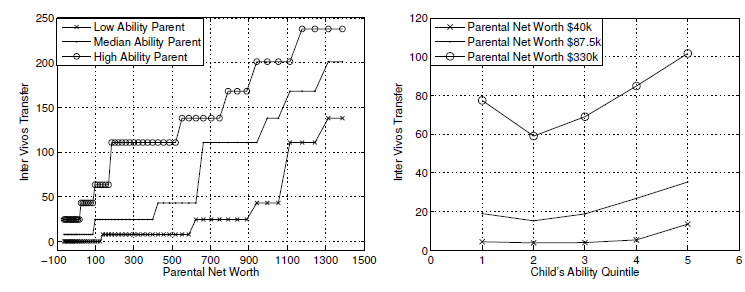
\includegraphics[width=115mm]{Figure2.png}\\
\tiny{Note: Parental transfers to children as a function of: children's ability and parental wealth (left panel); parental wealth and parent's ability (right panel)}

\end{center}

\end{frame}

\begin{frame}{Intergenerational Persistence of Education and Income}
\begin{itemize}
\item In the model 46.4\% of those whose mother is a college graduate become college graduates themselves (similar in NLSY79 data). %47.2\%  
%\item 54.4\% of those for whom both parents are college graduates become college graduates themselves (55.3\% in NLSY79 data)
%\item Replicating these high degrees of persistence due to the inclusion of non cognitive traits and paternalism. 
\begin{itemize}
\item Non-cognitive skills are important because parental education leads
to improvements in these skills, which in turn reduces the psychic costs. %of college for children of educated parents. 
\item Paternalism increases the tendency for rich parents to ‘send’ their child to college. %and hence it augments one’s probability of attending college if parents are educated.
\end{itemize}
\item Chetty et al. (2014) use IRS tax data to study the relationship between the mean child income rank and parents’ income rank for cohorts of children born between 1971-1986, and estimate a linear regression slope between 0.25 and 0.35 for male children.  The model finds a slope of 0.315 using the same definition of pre-tax income averaged over ages 31-46 for both children and parents. %depending on the birth year.
\end{itemize}
\end{frame}


\begin{frame}{Parental Wealth and Educational Achievement}
\begin{center}
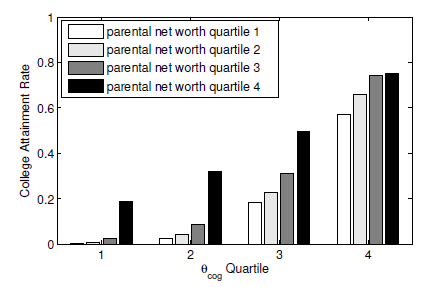
\includegraphics[width=100mm]{Figure3.png}\\
\tiny{Note: College attainment rate by cognitive ability and parental wealth: model simulations}

\end{center}
\end{frame}

%%%% Abbott slides model, estimation, policy experiments go here

%%%%%%%%%%%%%%%%%%%%%%%%%%%%%%%%%%%%%%%%%%%%%%%%%%%%%%%%%%%%%%%%
%%%%%%%%%%%%%%%%%%%%%%%%%%%%%%%%%%%%%%%%%%%%%%%%%%%%%%%%%%%%%%%%

\section{Policy Experiments}

\begin{frame}{Model Estimates Used for Policy Experiments}
\begin{itemize}
  \item Estimates two sets of policy experiments
    \begin{itemize}
    \item \textit{Randomizes} policies on high school graduates
      \item Examines the role of \textit{existing} federal financial aid
      \item Examines the role of \textit{marginal expansions} in financial aid \\[5mm]
    \end{itemize}
   \item Short-run partial equilibrium effects
   \begin{itemize}
  		\item Affects only a single cohort
        \item Policy announced just before inter vivos transfers $(j = 15)$
        \item Incorporates parent transfers and child's labor supply in college \\[5mm]
	\end{itemize}
	\item Long-run general equilibrium effects
   \begin{itemize}
  		\item Endogenous response of factor prices and alternative funding
        \item Budget balancing adjustments made by fiscal authority
        \item Estimates welfare changes expressed as percentage of lifetime consumption for a \textit{newborn} agent $(j = 0)$ with respect to initial conditions     
	\end{itemize}
\end{itemize}
\end{frame}

\begin{frame}{Removing Grants Reduces College Attainment}
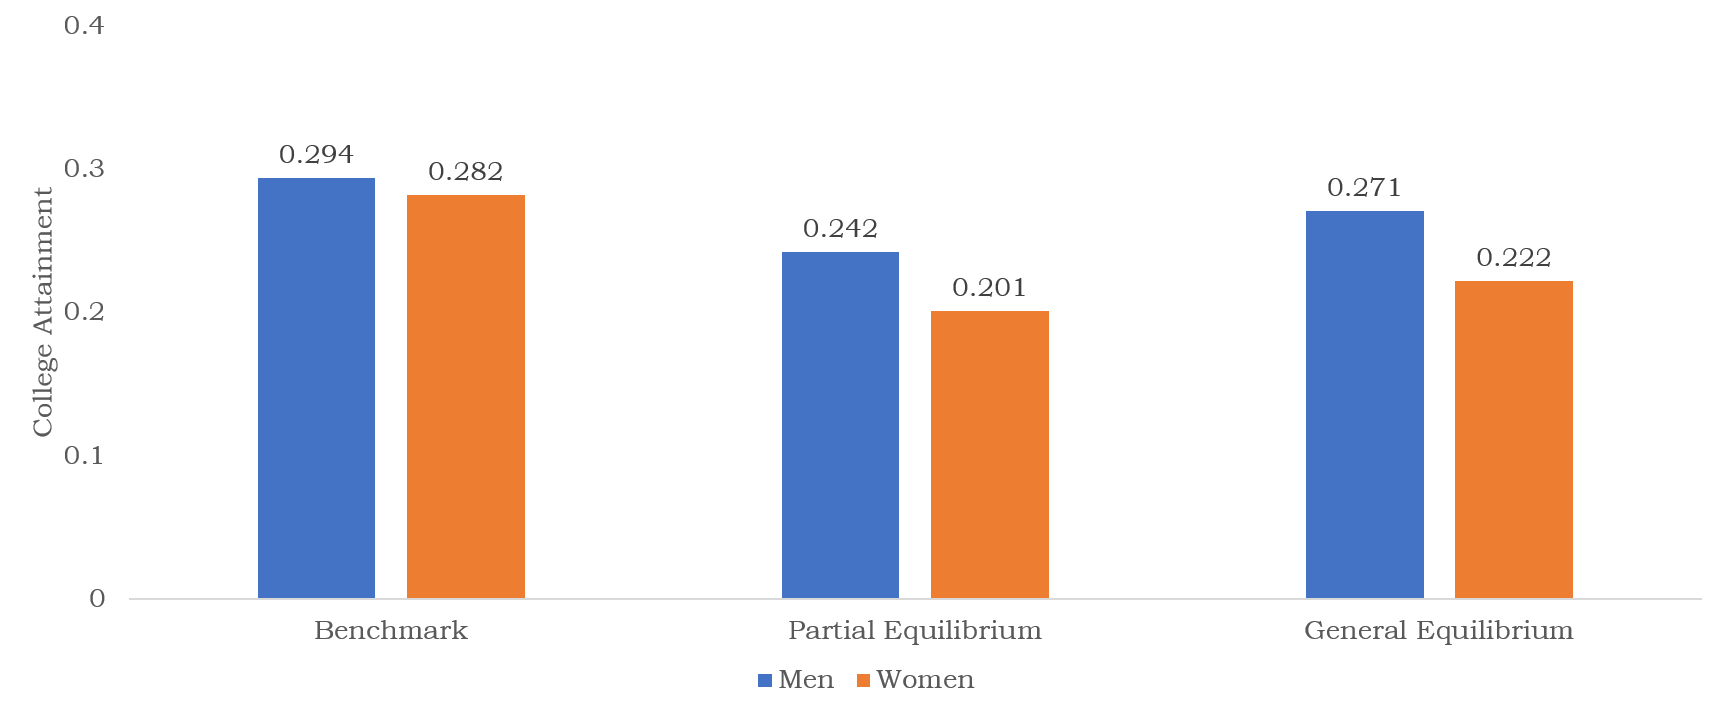
\includegraphics[width=\textwidth]{grantsattain.png}
\end{frame}

\begin{frame}{Removing Grants Alters Composition of Ability}
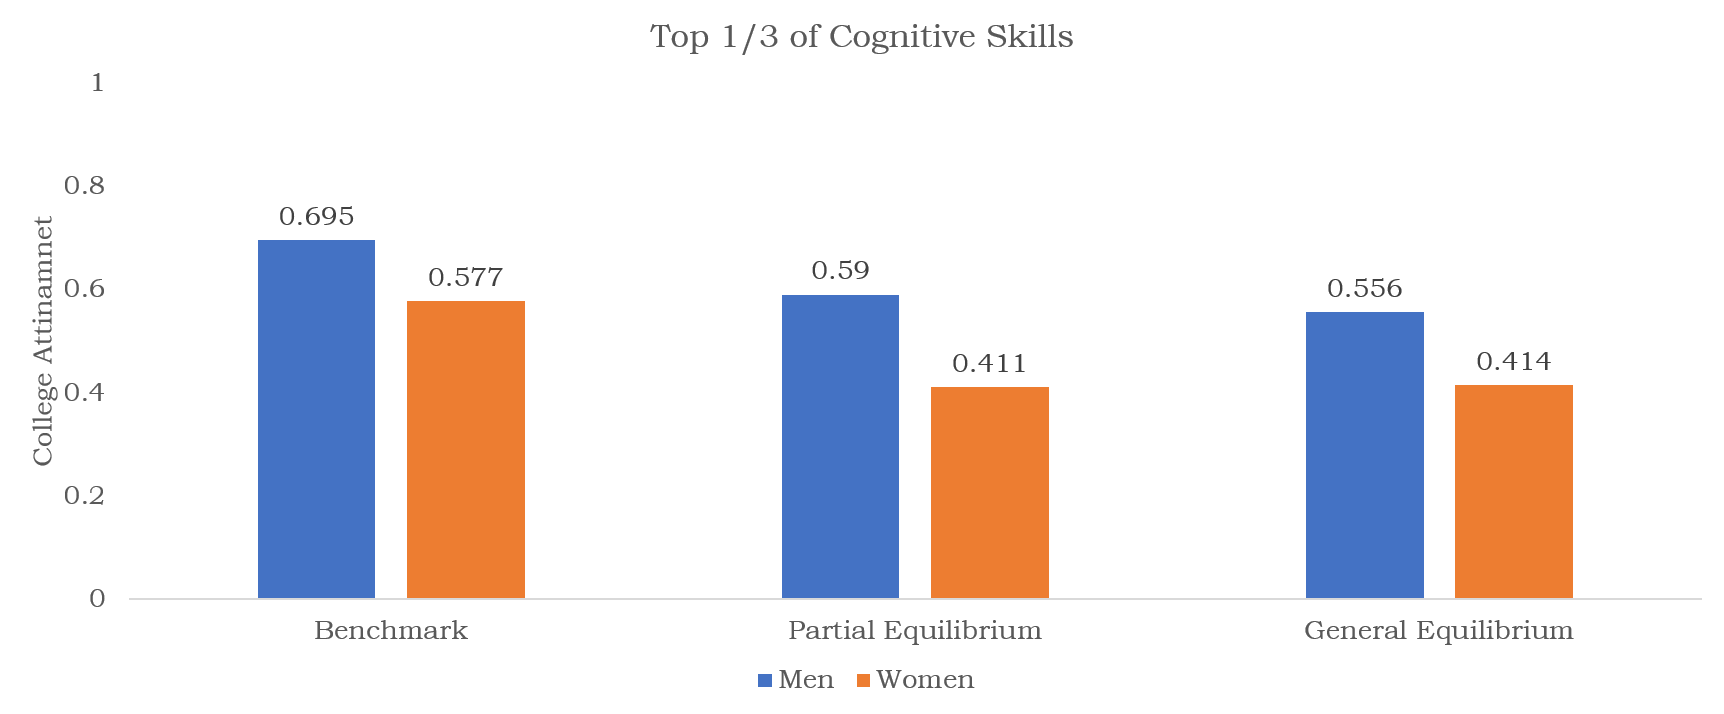
\includegraphics[width=\textwidth]{grantsskill.png}
\end{frame}

\begin{frame}{Removing Grants Increases Importance of Family Wealth}
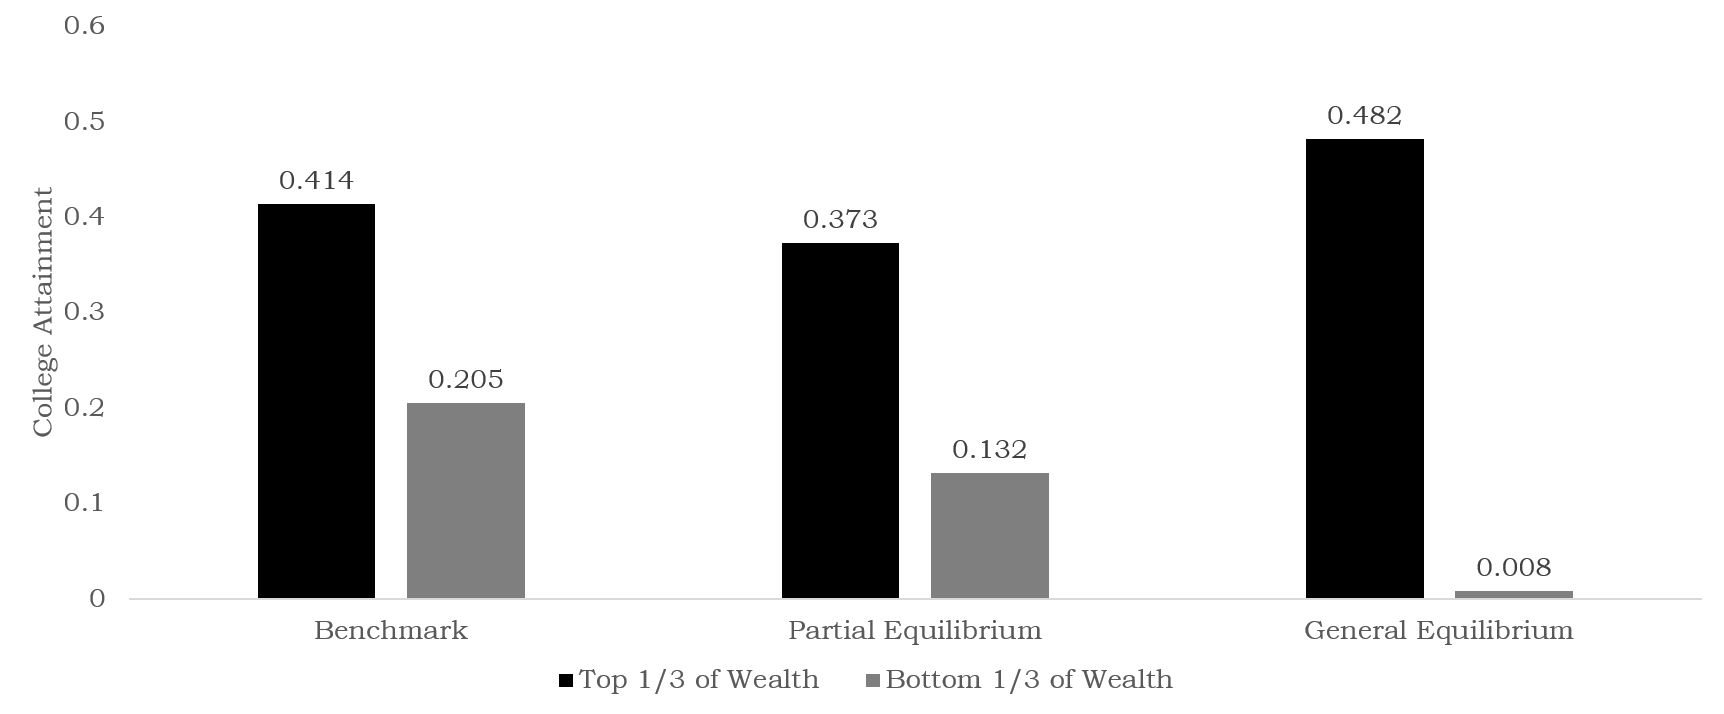
\includegraphics[width=\textwidth]{grantswealth.png}
\end{frame}

\begin{frame}{Labor lead to a decrease in output and welfare. and Transfers Increase}
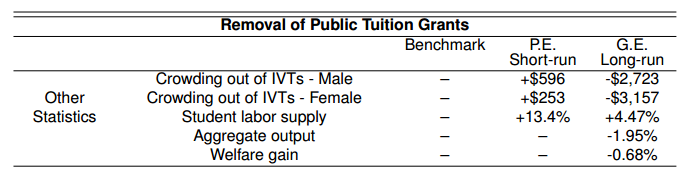
\includegraphics[width=\textwidth]{removegrants.png}
\begin{itemize}
\item Crowd out is the average change in IVTs given to children who are college graduates in both cases. \\[2mm]
\item IVTs increase in PE as families make up for grants \\[2mm]
\item Transfers lower in GE due to lower lifetime wealth \\[2mm]
\item Model does not allow for reductions in schooling effort associated with working while in college
\end{itemize}
\end{frame}

%\begin{frame}{Ex-Ante Welfare Loss is 0.7\%}
%\begin{itemize}
%\item Losses due to a lower average consumption and more %unequal initial conditions
%\item Average productivity suffers from lower schooling %levels and worse sorting of children by ability. 
%\item Inequality in initial conditions deteriorates
%\begin{itemize}
%\item Grants provide insurance against low draws on parental characteristics. \item The rise in the college premium redistributes against low-income low-ability individuals who do not enroll in college.
%\end{itemize}
%\item There is a large offsetting welfare effect due to a reduction in average volatility of consumption in the population
%\end{itemize}
%\end{frame}

\begin{frame}{Removing Loans also Reduces Attainment}
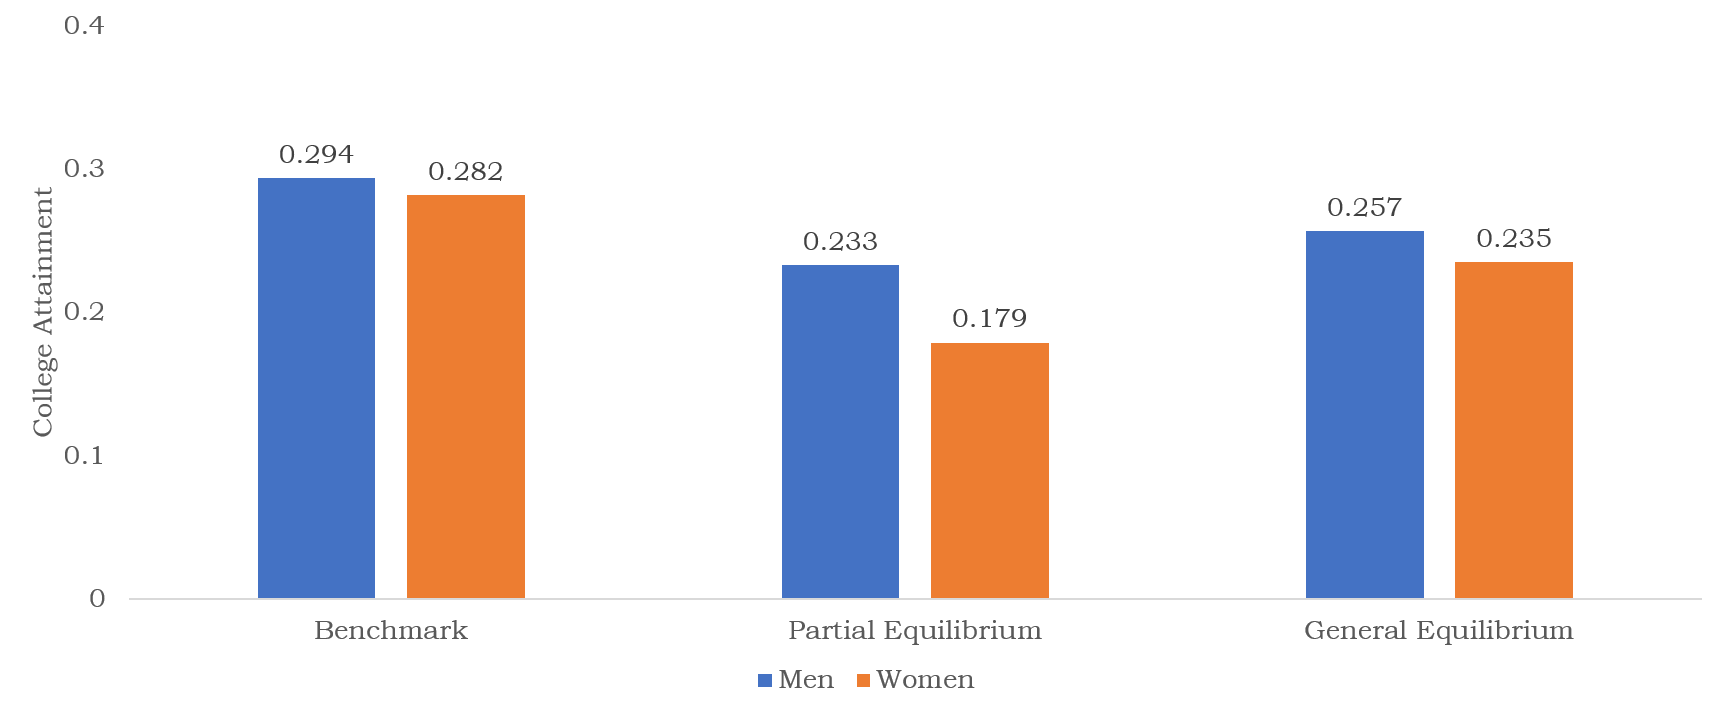
\includegraphics[width=\textwidth]{loansattain.png}

Only the richest group (q = 3) is able to borrow to finance college
\end{frame}

\begin{frame}{Worsening of Selection on Ability}
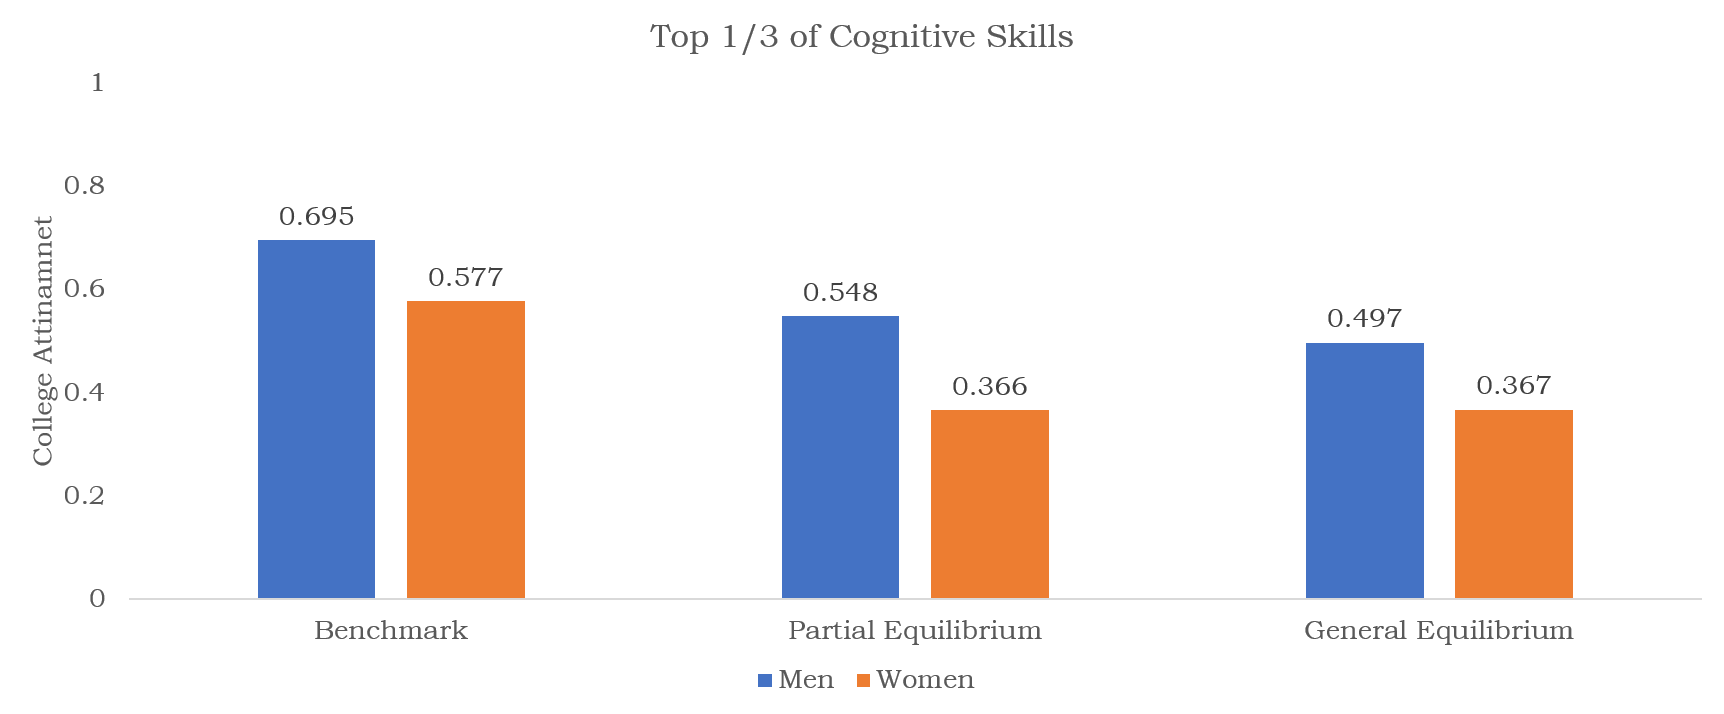
\includegraphics[width=\textwidth]{loansskills.png}
\end{frame}

\begin{frame}{Worsening of Selection on Wealth}
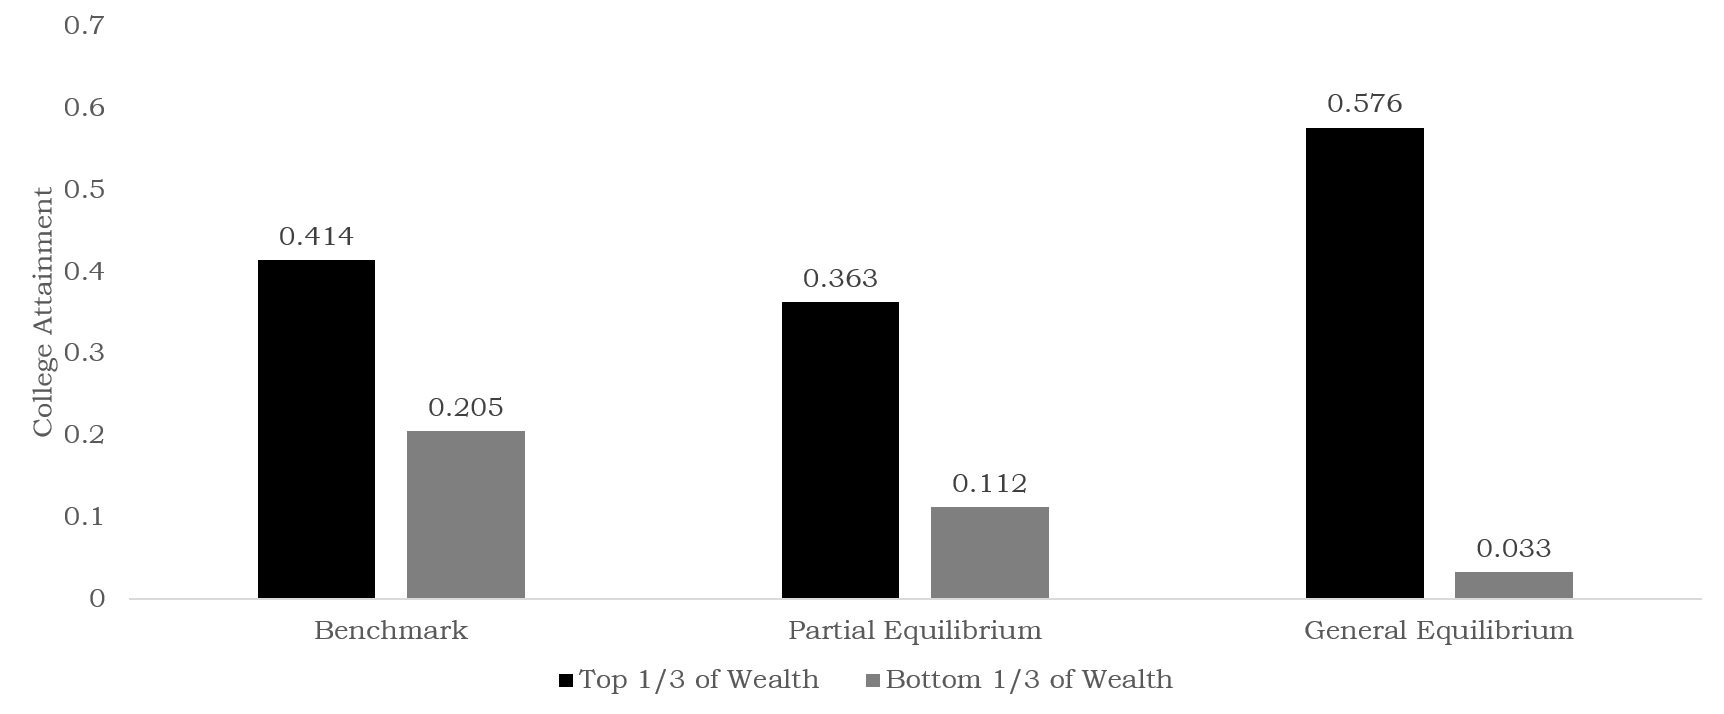
\includegraphics[width=\textwidth]{loanswealth.png}
\end{frame}

\begin{frame}{Larger Crowd out of IVT's from Loans in Long Run}

\begin{table}[]
\centering
\label{my-label}
\begin{tabular}{|l|l|l|}
\hline
                 & \multicolumn{2}{l|}{Estimated Policy Effects in Long-Run} \\ \hline
                 & Removal of Grants      & Removal of Loans     \\ \hline
Crowd out of IVTs - Male & -\$2,723                & +\$3,740              \\ \hline
Crowd out of IVTs - Female & -\$3,157                & +\$2,199              \\ \hline
\end{tabular}
\end{table}
\end{frame}

\begin{frame}{Both Experiments Reduce Welfare}

\begin{table}[]
\centering
\label{my-label}
\begin{tabular}{|l|l|l|l|}
\hline
                 & \multicolumn{3}{l|}{Estimated Policy Effects} \\ \hline
                 & Grant Removal      & Loan Removal & Removing Both    \\ \hline
Output & -1.95\%                & -2.95\%          & -4.5\%    \\ \hline
Welfare Gain     & -0.68\%                & -0.65\%           & -1.85\%   \\ \hline
\end{tabular}
\end{table}

\begin{itemize}
\item Welfare and output effects are driven by changes in sorting \\[2mm]
\item Cumulative effects of removing both policies is greater
\item Reinforcing patterns emerge through the intergenerational transmission of skills \\[2mm]
\begin{itemize}
\item When the fraction of college educated women declines, cumulative psychic costs of going to college rise
\end{itemize}
\end{itemize}
\end{frame}

\begin{frame}{Considers Four Possible Expansions}
\begin{enumerate}
\item Remove credit constraint ('unconstrained economy')
\begin{itemize}
\item All debts must be repaid at $r^{-}$ by retirement.
\item Federal grant program is left unchanged \\[5mm]
\end{itemize}
\item Increase grants by \$1,000 per year \\[5mm]
\item Increase grants proportionally with means. \\[5mm]
\item Increase grants proportionally to cognitive skills. \\[5mm] 
\end{enumerate}
\end{frame}

\begin{frame}{Unconstrained Economy has Modest Effects}
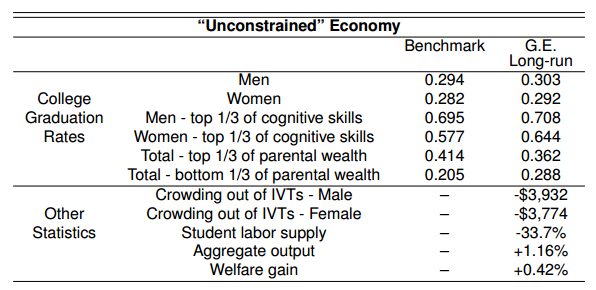
\includegraphics[width=\textwidth]{unconstrained.png}
\end{frame}

\begin{frame}{Similar Pattern from All Grant Expansions}
\begin{table}[]
\centering
\resizebox{\textwidth}{!}{\begin{tabular}{|l|l|l|l|l|}
\hline
                              &           & \multicolumn{3}{l|}{Long-run General Equilibrium Response} \\ \hline
                              & Benchmark & Flat Expansion      & Means-Tested      & Merit-Based      \\ \hline
Men                           & 0.294     & 0.320               & 0.325             & 0.303            \\ \hline
Women                         & 0.282     & 0.293               & 0.297             & 0.296            \\ \hline
Top 1/3 of Cog Skills         & 0.637     & 0.647               & 0.659             & 0.681            \\ \hline
Top 1/3 of Parental Wealth    & 0.414     & 0.401               & 0.379             & 0.399            \\ \hline
Bottom 1/3 of Parental Wealth & 0.205     & 0.239               & 0.283             & 0.237            \\ \hline
\end{tabular}}
\end{table}
\end{frame}

\begin{frame}{Efficiency Gains Driven by Selection and Enrollment}
\begin{table}[]
\centering
\begin{tabular}{|l|l|l|l|}
\hline
                 & \multicolumn{3}{l|}{Long-run General Equilibrium Response} \\ \hline
                 & Flat Expansion      & Means-Tested      & Merit-Based      \\ \hline
Aggregate Output & +0.46\%             & +0.66\%           & +0.57\%          \\ \hline
Welfare Gain     & +0.32\%             & +0.40\%           & +0.31\%          \\ \hline
\end{tabular}
\end{table}
\end{frame}

%\begin{frame}{Crowd-out Mitigates Policy Effects}
%\begin{table}[]
%\centering
%\begin{tabular}{|l|l|l|l|}
%\hline
%                     & \multicolumn{3}{l|}{Long-run General Equilibrium Response} \\ \hline
%                     & Flat Expansion      & Means-Tested      & Merit-Based      \\ \hline
%Crowding out IVTs    & -\$1,353            & -\$791            & -\$1,619         \\ \hline
%Student Labor & -3.22\%             & -5.17\%           & -3.90\%          \\ \hline
%\end{tabular}
%\end{table}
%\end{frame}

\begin{frame}{Heterogeneous Welfare Effects from Means-tested Grants}

\begin{table}[]
\centering
\label{my-label}
\begin{tabular}{llll}
\multicolumn{4}{c}{Distribution of Welfare Changes}                                                                      \\ \hline
\multicolumn{1}{|l|}{}      & \multicolumn{2}{c}{$\theta_{cog}$ tercile}                 & \multicolumn{1}{l|}{}        \\ \hline
\multicolumn{1}{|l|}{}      & \multicolumn{1}{l|}{1}       & \multicolumn{1}{l|}{2}       & \multicolumn{1}{l|}{3}       \\ \hline
\multicolumn{1}{|l|}{q = 1} & \multicolumn{1}{l|}{0.71\%}  & \multicolumn{1}{l|}{2.91\%}  & \multicolumn{1}{l|}{5.57\%}  \\ \hline
\multicolumn{1}{|l|}{q = 2} & \multicolumn{1}{l|}{-5.22\%} & \multicolumn{1}{l|}{-5.43\%} & \multicolumn{1}{l|}{-2.19\%} \\ \hline
\multicolumn{1}{|l|}{q = 3} & \multicolumn{1}{l|}{-7.64\%} & \multicolumn{1}{l|}{-4.90\%} & \multicolumn{1}{l|}{-2.14\%} \\ \hline
\end{tabular}
\end{table}

\end{frame}

\begin{frame}{Policy Experiment Conclusions}

\begin{itemize}
\item The authors corroborate the results from Heckman et al (1998), Lee (2005), and Lee and Wolpin (2006) 
\item In the long-run prices adjust and the aggregate effects of policies are mitigated
\begin{itemize}
\item Throughout all of their experiments, changes in college attainment in the long-run GE are roughly half the size of the the short-run PE case.
\item They do find sizable benefits for certain groups such as high ability/low income girls
\end{itemize}
\item Welfare changes are associated with changes in sorting
\item Significant heterogeneity in crowd-out
\end{itemize}
\end{frame}

%%%%%%%%%%%%%%%%%%%%%%%%%%%%%%%%%
\section{Discussion and Other Recent Work}
\begin{frame}{Contribution}
\begin{itemize}
\item General equilibrium life cycle model that shows the following: 
\begin{itemize}
\item Intergenerational transfer through paternalism and altruism and endogenous transmission of skill endowment
\item Importance of cognitive and non-cognitive skills for psychic costs 
\item Role of parental transfers, private borrowing, and labor supply in college for financing education
\item Imperfect substitution between gender and education groups in production function
\end{itemize}
\item Policy experiments show that financial aid system improves welfare.
\item Removing current financial aid system would reduce GDP by 4-5\%.
\item Further expansions of loans or grants would not increase welfare.
\end{itemize}
\end{frame}

\begin{frame}{Our conclusions (1/2)}
The model is extremely complicated making the impact of particular features of the model hard to interpret. Does it need to be?
\begin{itemize}
\item General equilibrium vs partial equilibrium framework
\begin{itemize} 
\item Abbott shows that PE effects are moderated in the GE setting because decision makers respond to changes in prices over time
\item Consistent with earlier work, eg. Heckman, Lochner and Taber (1998)
\end{itemize}
\item Multiple generations vs single generation models
\begin{itemize}
\item Keane and Wolpin (2001) and Johnson (2011) model single generation models (with parent transfers conditional on parent education and child schooling decision) and reach similar conclusions
\item Possible that, if taking states at age 16 as given, modeling intergenerational relationships doesn't add much to the analysis
\end{itemize}

\end{itemize}
\end{frame}

\begin{frame}{Our conclusions (2/2)}
\begin{itemize}
\item Modeling of Psychic costs is not clear; Using just two measures of skills (cognitive and non-cognitive skills) they are able to account for a much larger portion of variation in the college decision as in the rest of the literature
\item How important is gender heterogeneity? It is not modeled in many previous papers.
\item Show women having high labor supply elasticity throughout child's first 16 years but Blundell (2017) showed us this high elasticity is mostly during the child's early years, prior to entering school
\item How would including variation in college quality and college tuition affect the results? \\
There is evidence that students with lower wealth parents substitute away from high quality / high tuition schools due to credit constraints; this has implications for IGC which are ignored here
\end{itemize}
\end{frame}

%%%%%%%%%%%%%%%%%%%%%%%%%%%%%%%%%%%%%%%%%%%%%%%%%%%%%%%%%%%%%%%%
%%%%%%%%%%%%%%%%%%%%%%%%%%%%%%%%%%%%%%%%%%%%%%%%%%%%%%%%%%%%%%%%
%%%%%%%%%%%%%%%%%%%%%%%%%%%%%%%%%%%%%%%%%%%%%%%%%%%%%%%%%%%%%%%%

\begin{frame}
Briefly discuss two additional recent papers on intergenerational transfers between parents and children 
\begin{itemize}
\item  Lee, Sang Yoon and  Ananth Seshadri. (2015). ``On the Intergenerational Transmission of Economic Status.'' Working Paper, University of Wisconsin. 
\item Caucutt, Elizabeth, Lance Lochner and Youngmin Park. (2015). "Correlation, Consumption, Confusion, or Constraints: Why do Poor Children Perform so Poorly?" Scandinavian Journal of Economics, 119:102-147.
\end{itemize}
\end{frame}

%%%%%%%%%%%%%%%%%%%%%%%%%%%%%%%%%%%%%%%%%%%%%%%%%%%%%%%%%%%%%%%%
%%%%%%%%%%%%%   Lee Seshadri     %%%%%%%%%%%%%%%%%%%%%%%%%%%%%%%

\subsection{Lee and Seshadri (2016)} 

\begin{frame}{Lee and Seshadri (2016)}
\begin{itemize}
\item Similar to Abbott et al. in that they create a complex multi-generation model with incomplete markets and government transfers.
\item Goal is to model both intergenerational mobility and cross-sectional inequality
\item Focus on the impact of early childhood investments on income inequality as a primary mechanism for inequality
\item Use PSID - CDS data
\item Run policy experiments, make welfare predictions
\end{itemize}
\end{frame}

\begin{frame}{Lee and Seshadri (2016)}
Differences from Abbott et al. (1/2): 
\begin{itemize}
\item Model human capital formation
\begin{itemize}
\item Multiple periods of child investment (6 year periods; childhood lasts 4 periods) 
\hyperlink{lstime}{\beamerbutton{Timeline}}
\item Allow for both time and consumption goods investments in children
\item Convert time to opportunity cost using parent's hourly wage rate
\item Childcare goods: related to cognitive skill development; drop observations with no spending reported; include public school costs
\item Ben Porath model (OJT) skill formation while working 
\item Test scores as a proxy for child skills when enter the labor market. No measure of non-cognitive skills
\end{itemize}
\end{itemize}
\end{frame}

\begin{frame}{Lee and Seshadri (2016)}
Differences from Abbott et al. (2/2): 
\begin{itemize}
\item No marriage or gender, single parent-single child
\item One main result from Abbott is that child work during college responds to the policy; this is omitted in this paper because they assume children do not work while attending college
\item Altruism for children modeled but not paternalism (there are no conditional on education level transfers)
\item Model government consisting of: progressive taxes on income which subsidize welfare payments; education subsidies; social security 
\end{itemize}

\end{frame}

%Include any tables/figures? Time/$ investment Figure 7 is interesting

\begin{frame}{Lee and Seshadri (2016) - Findings}
\begin{itemize}
\item Decompose variance in child lifetime earnings and lifetime wealth:
\begin{itemize} 
\item 74\%, 73\% explained by age 24 (whether or not went to college, learning ability and human capital accumulated, parent transfer) and omitting the college decision does not change this estimate meaning college decision is not very important in independently explaining earnings/wealth variance
\item 71\%, 72\% explained at child's birth (age 0-5)
\item 22\%, 49\% explained by parents' states age 24-29
\item 19\%, 34\% explained by grandparents' states  age 24-29
\end{itemize}
\end{itemize}
%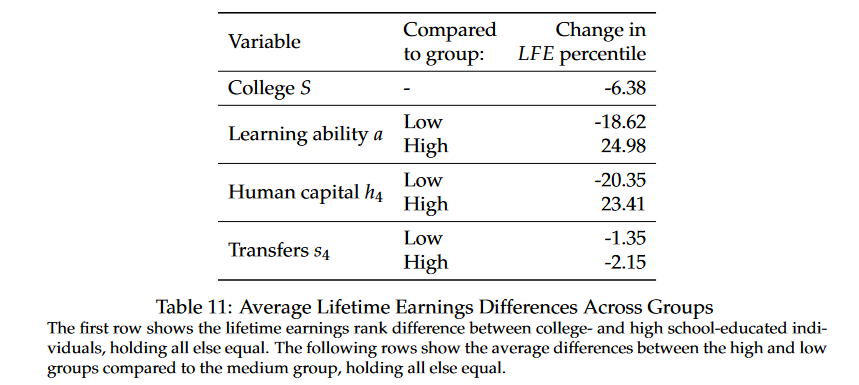
\includegraphics[width=\textwidth]{leeseshadri1.PNG}
\end{frame}

\begin{frame}{Lee and Seshadri (2016) - Findings}
\begin{itemize}
\item Model dynamic complementarity in early childhood education. Parents cannot fully substitute later investments with early investments.
\item Reducing borrowing constraints of families with young children, rather than policies focused on constraints during college, would have large impact in increasing economic mobility across generations.
\item Evidence that while model from Abbott shows that current college financial aid system is optimal, focusing on college ignores the potential to reduce IGC through investments in early childhood education.
\end{itemize}
\end{frame}

%%%%%%%%%%%%%%%%%%%%%%%%%%%%%%%%%%%%%%%%%%%%%%%%%%%%%%%%%%
%%%%%%%%%%%%%%% Yuvraj's slides - begin %%%%%%%%%%%%%


%\begin{frame}
%\frametitle{Setting up Abbott et al.}
%Abbott et al. model a lifecycle general equilibrium human capital investment model to study welfare impact of financial aid policies
%\begin{itemize}
%\item Ability correlation: Child's cognitive and non-cognitive ability draw from the mother
%\item Consumption Value of Investment: Parents are altruistic and paternalistic  
%\item Systematic bias: Assumes no income dependent information friction
%\item Credit constraints: Explicitly model credit constraints facing an agent when making education/work decisions

%\end{itemize}
%\end{frame}

%\begin{frame}{Introduction}
%Caucutt (2017) 4 Stylized Facts re Child Development
%\begin{itemize}
%\item Returns to early childhood marginal investments are higher than the returns to savings for low income children
%\item Returns to early investments are lower for high income children than for low income children 
%\item Exogenous increases in parent income result in greater investment in children and improved child outcomes
%\item Increases in income when children are young are more beneficial than increases in income for older children
%\end{itemize}
%\end{frame}

\subsection{Caucutt et al. (2015)} 

\begin{frame}
\frametitle{Caucutt}
Uses a dynamic human capital investment model to study four investment based mechanisms driving income based skill gaps 

\begin{itemize}
\item Ability correlation: High ability parents might have high ability children 
\item Consumption value of investment: Parents derive utility from investing in children
\item Information Frictions: Poor parents might have incorrect beliefs about returns on child investment
\item Credit constraints: Limits on capacity to borrow might decrease investment
\end{itemize}
\end{frame}

\begin{frame}
\frametitle{Caucutt}
Focus on the mechanisms to explain the following findings from literature:

\begin{itemize}
\item Higher returns on investment in children compared to savings for poor children
\item Returns on marginal investment decreasing in income
\item Increase in income lead to increase in investment
\item Timing of this income increase matters - higher returns at early age
\end{itemize}
\end{frame}

\begin{frame}
\frametitle{Caucutt}
Key insights from the model:
\begin{itemize}
\item Positive consumption value of investment leads to lower marginal return to investment as parents invest beyond the income maximizing amount. This is increasing in parental income.
\item Expected marginal returns decreasing in income in case of uncertainty in return
\item Bias in belief about returns leads to lower marginal return for both rich and poor children as families tend to underinvest 
\item Credit constraints can explain the low investment and high marginal return in case of poor children
\end{itemize}
\end{frame}

\begin{frame}
\frametitle{Abbott improving on Caucutt}
Abbott et al improves on Caucutt in many ways
\begin{itemize}
\item Explicitly model gender differences in investment and outcomes
\item Borrowing constraints are allowed to depend on household income and differ in different time periods  
\item Differentiates between cognitive and non-cognitive ability
\item Importantly, attempts to differentiate between altruism and paternalism

\end{itemize}
\end{frame}



%%%%%%%%%%%%%%%%%%%%%%%%%%%%%%%%%%%%%%%%%%%%%%%%%%%%%%%%%%%%%%%%
%%%%%%%%%%%%%%%%%%%%%%%%%%%%%%%%%%%%%%%%%%%%%%%%%%%%%%%%%%%%%%%%

\section{References}
\begin{frame}{References}
\begin{footnotesize}
\begin{itemize}
\item Abbott, Brant, Giovanni Gallipoli, Costas Meghir, and Giovanni Violante. (2016). "Education Policy and Intergenerational Transfers in Equilibrium," Under revision, Journal of Political Economy. 

\item Becker, Gary S. and Tomes, Nigel. (1986). ``Human Capital and the Rise and Fall of Families.'' Journal of Labor Economics, 4(3, Part 2): S1-S39.

\item Caucutt, Elizabeth, Lance Lochner and Youngmin Park. (2015). "Correlation, Consumption, Confusion, or Constraints: Why do Poor Children Perform so Poorly?" Scandinavian Journal of Economics, 119:102-147.

\item Chetty, Raj, Nathaniel Hendren, Patrick Kline, and Emmanuel Saez. ``Where is the Land of Opportunity? The Geography of Intergenerational Mobility in the United States.'' Quarterly Journal of Economics 129(4): 1553-1623, 2014.

%\item Chetty, Raj, David Grusky, Maximilian Hell, Nathaniel Hendren, Robert Manduca, Jimmy Narang. ``The Fading American Dream: Trends in Absolute Income Mobility Since 1940.'' National Bureau of Economic Research Working Paper No. 22910, 2016

%\item Haider, Steven J, Kathleen McGarry. ``Parental Investments in College and Later Cash Transfers.'' Working Paper. September 2002.

\item Heckman, James J, Stefano Mosso. ``The Economics of Human Development and Social Mobility.'' Annu. Rev. Econ. 2014. 6:689:733.

\item  Lee, Sang Yoon and  Ananth Seshadri. (2015). ``On the Intergenerational Transmission of Economic Status.'' Working Paper, University of Wisconsin. December, 2016.

%\item The College Board. ``Trends in Student Aid 2016''. \url{https://trends.collegeboard.org/sites/default/files/2016-trends-student-aid_0.pdf}

\end{itemize}
\end{footnotesize}
\end{frame}

\begin{frame}[label=supplemental]{Externally Set Parameters}
\hyperlink{Return1}{\beamerbutton{Return}}
\begin{center}
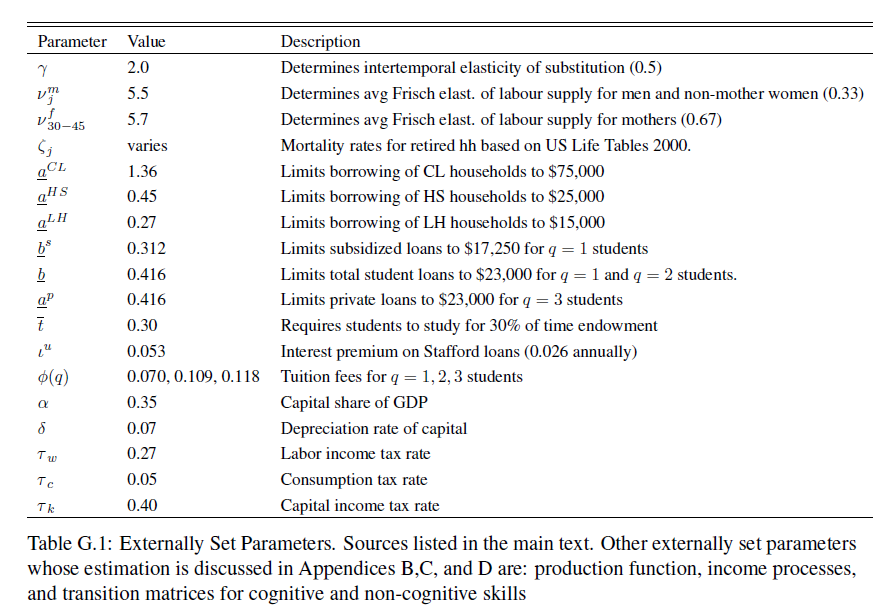
\includegraphics[width=100mm]{Image1.png}
\end{center}
\end{frame}

\begin{frame}[label=supplemental1]{Externally Set Parameters}
\hyperlink{Return1}{\beamerbutton{Return}}
\begin{center}
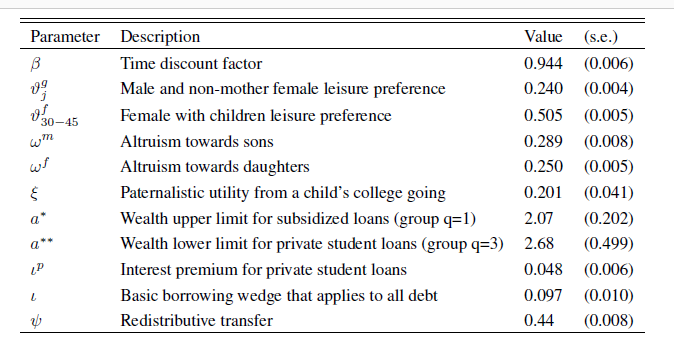
\includegraphics[width=100mm]{Image2.png}
\end{center}
\end{frame}

\begin{frame}[label=supplemental2]{Other estimates by Method of moments}
\hyperlink{Return1}{\beamerbutton{Return}}
\begin{center}
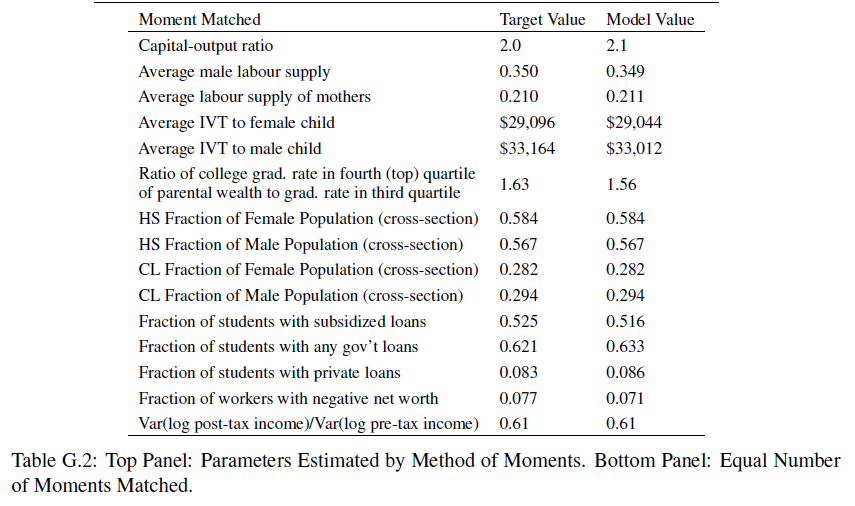
\includegraphics[width=100mm]{Image3.png}
\end{center}
\end{frame}


\begin{frame}[label=Production1]{Aggregate Production Function}
\hyperlink{Return1}{\beamerbutton{Return}}
\begin{itemize}
\item Current Population Survey (CPS) for 1968-2001. Sample includes the adult universe.
\item Perfect competition. Total wage bill (billions of dollars for the three education groups, as well as for their subsets by gender) divided by the (normalized) marginal product of human capital estimated from PSID data (The Panel Study of Income Dynamics).
\item Assumption of iso-elasticity (tested in Appendix).
\item Share parameters vary over time. Shares are normalized to sum to one at every t.
\item Gender-specific parameters: $log(\frac{\bar{\omega}_t^{fe}}{\bar{\omega}_t^{me}})=log(\frac{s_t^{fe}}{s_t^{me}})+\chi log(\frac{H_t^{fe}}{H_t^{me}})$. This equation holds for all groups of education.
\item Education-specific parameters: $log(\frac{\bar{\omega}_t^{CL}}{\bar{\omega}_t^{HS}})=log(\frac{s_t^{CL}}{s_t^{HS}})+\rho log(\frac{H_t^{CL}}{H_t^{HS}})$.

\end{itemize}
\end{frame}


\begin{frame}{Aggregate Production Function}

\begin{table}[H]
\caption {Production estimates} \label{tab:title} 
\begin{center}
 \begin{tabular}{ c | c | l }
  \hline
   Parameter & Estimation & Comments \\ \hline
   $\rho$ & 0.7 & \tiny{Elasticity of substitution between education aggregates to 3.3} \\ 
 $\chi$ & 0.45 & \tiny{‘Education-conditional’ elasticity of 1.8 between men and women} \\

            $s^{LH}$ & 0.16 & \tiny{Year 1999} \\
            $s^{HS}$ & 0.38 & \tiny{Year 1999}   \\
            $s^{CL}$ & 0.46 &  \tiny{Year 1999}  \\
 
            $s^{f,LH}$ & 0.34 &  \tiny{Gender weights for different education
groups, Year 1999}  \\
            $s^{f,HS}$ & 0.40 &  \tiny{Year 1999}  \\
            $s^{f,CL}$ & 0.38 &  \tiny{Year 1999}  \\
               
 %Share no suma 1 ??? 

    \hline
  \end{tabular}
\end{center}
\end{table}

\begin{itemize}
\item Log college/high-school wage differential of 0.58 
\item Log high-school graduate/dropout wage differential of 0.37, consistent with literature.
\item Education-conditional’ elasticity of 1.8 between men and women
\item Elasticity of substitution between education aggregates to 3.3
%25Many estimates in the literature are based on a coarser two-type skilled/unskilled classification for labor, with no
gender differences. Katz and Murphy (1992) estimate the elasticity of substitution to be 1.41; Heckman et al. (1998a)
report a favorite estimate of 1.44. Card and Lemieux (2001) obtain an elasticity of substitution between college and high
school workers of about 2.5; however, their estimated elasticity, when accounting for imperfect substitutability across age
groups, ranges between 4 and 6. Finally, using a nested specification with three human capital types Goldin and Katz
(2007) suggest a preferred elasticity between college and non-college workers of 1.64.
%\item Estimation of IV approach to control endogeneity of human capital inputs (lagged regressors).
\end{itemize}
    
\end{frame}


\begin{frame}[label=Income1]{Income Process and the Impact of Ability on Earnings}
\hyperlink{Return4}{\beamerbutton{Return}}
\begin{itemize}
\item Individual wage dynamics depend on age, gender, education and abilities (only cognitive). Correct for selection into work.
\item Idiosyncratic labor productivity process: $\epsilon_j^{g,e}=\lambda^{g,e}log\theta_{cog} + z_j^{g,e} $
\item $z_j^{g,e} =\varrho^{g,e}z_{j-1}^{g,e} + \eta_j^{g,e}$, where $\eta_j^{g,e}\sim^{iid} N(0, \sigma_{\eta}^{g,e})$
\item $\lambda^{g,e}$: impact of cognitive skills on wages, $\varrho^{g,e}$: persistence of idiosyncratic productivity shocks, $ \sigma_{\eta}^{g,e}$: variance of the shock that vary across gender and education. 
\item Heterogeneity in returns to schooling will in part drive differences in education choices between men and women and across ability groups.
\end{itemize}

\end{frame}

\begin{frame}[label=Transmission2]{Intergenerational Transmission of Cognitive Skills}
\hyperlink{Return5}{\beamerbutton{Return}}

\begin {table}[H]
\caption {Ability transition matrix across skill quintiles } \label{tab:title} 
\begin{center}
  \begin{tabular}{c | c  c  c  c  c}
      \hline
     & \multicolumn{5}{c}{Children} \\ 

    Mother & 1 & 2 & 3 & 4 & 5 \\ \hline
1&0.455 & 0.238& 0.197& 0.065& 0.047 \\ 
2 &0.258& 0.242& 0.242 &0.157 &0.110\\ 
3& 0.160& 0.223& 0.271 &0.190 &0.157\\ 
4 &0.114& 0.171& 0.257& 0.209 &0.249\\ 
5 &0.072& 0.076 &0.195& 0.242 &0.415\\  \hline
\end{tabular}
\end{center}

\tiny{Notes: Ability transition probabilities, by quintile (NLSY79). Quintile 1 is the lowest ability, quintile 5 is the highest.}
\end {table}



\end{frame}

\begin{frame}[label=Transmission1]{Intergenerational Transmission of Cognitive and Non-Cognitive Skills}
\hyperlink{Return5}{\beamerbutton{Return}}

\begin {table}[H]
\caption {Non-cognitive Ability Transitions} \label{tab:title} 
\begin{center}
  \begin{tabular}{c | c  c  c  c  c}
      

\multicolumn{6}{c}{\tiny{Children Conditional Probabilities of Non-Cognitive Tercile 1 Child’s Cognitive Quintile}} \\

\hline
Mother’s Edu& 1& 2& 3& 4 & 5\\ \hline
HSD& 0.585 &0.453& 0.350 &0.311& 0.189\\
HSG& 0.527 &0.418 &0.266 &0.235& 0.178\\
CLG &0.578& 0.388& 0.289 &0.201& 0.139\\\hline

\multicolumn{6}{c}{\tiny{Children Conditional Probabilities of Non-Cognitive Tercile 2 Child’s Cognitive Quintile}}\\
HSD & 0.297 &0.367& 0.339 &0.316& 0.347\\
HSG & 0.362 &0.330 &0.386 &0.333 &0.318\\
CLG &0.283& 0.343 &0.353& 0.356& 0.337\\\hline

\multicolumn{6}{c}{\tiny{Children Conditional Probabilities of Non-Cognitive Tercile 3 Child’s Cognitive Quintile}}\\
HSD & 0.118 &0.180& 0.311 &0.372 &0.464\\
HSG &0.111 &0.252 &0.348 &0.432 &0.504\\
CLG &0.139& 0.270 &0.358 &0.443 &0.525\\\hline


\end{tabular}
\end{center}
\tiny{Notes: Each cell reports the conditional probability of the child being
in the non-cognitive skill tercile corresponding to that table section. (NLSY79). Tercile 1 is the lowest, tercile 3 is the highest.}

\end{table}

\end{frame}

\begin{frame}[label=Income2]{Income Process and the Impact of Ability on Earnings}
\hyperlink{Return4}{\beamerbutton{Return}}

\begin {table}[H]
\caption {Estimated parameters of the process for individual efficiency units $\epsilon_j^{g,e}$
 (NLSY79)} \label{tab:title} 
\begin{center}
  \begin{tabular}{c | c | c | c }
      \hline
  Parameter & Less than HS & HS graduate & College graduate  \\ \hline
 $\varrho^m$  &  0.955 & 0.952 & 0.966  \\ 
  $\sigma_{\eta}^{m}$  & 0.015  & 0.017& 0.017 \\ 
   $\sigma_{z0}^{m}$  & 0.037& 0.059 & 0.094  \\ \hline
      $\varrho^{f}$  & 0.852  & 0.953 &  0.983\\ 
   $\sigma_{\eta}^{f}$  &  0.025& 0.019& 0.018  \\ 
   $\sigma_{z0}^{f}$  & 0.035 & 0.041 & 0.076   \\ 

              \hline
  \end{tabular}
\end{center}
\end {table}

\begin{itemize}
\item Shocks are very persistent, close to random walk for all but females with less than HS ($\varrho$).
\item Variance of initial productivity ($\sigma_{z0}$) increases with education for women, and more for men. Uncertainty difficult to insure against, since at young ages individuals tend to be wealth-poorer. %(Note: mean of the shock set as 0.)

\end{itemize}
\end{frame}
%%%%%%%%%%%%%%%%%%%%%%%%%%%%

\begin{frame}[label=Psychic1]{Eliminating Cross-Sectional Variation in Psychic Costs}
\hyperlink{Return6}{\beamerbutton{Return}}

\begin {table}[H]
\caption {Sensitivity of Enrollment to Psychic Costs Variation} \label{tab:title} 
\begin{center}
  \begin{tabular}{c | c  c  c  c  c}
    
\multicolumn{6}{c}{\textbf{Baseline Model}} \\
 
  & \multicolumn{5}{c}{Cognitive quintile} \\ 

Non cognitive tercile  & 1 & 2& 3& 4& 5\\\hline

1   & 0.087 & 0.114& 0.166& 0.298& 0.648\\
2 & 0.094& 0.125 &0.177 &0.334 &0.725\\
3 & 0.106 & 0.142 &0.193 &0.399 &0.806\\\hline

\multicolumn{6}{c}{\textbf{No Psychic Cost Variation}} \\ \hline


 & \multicolumn{5}{c}{Cognitive quintile} \\ 
Non cognitive tercile  & 1& 2 &3 &4 &5\\\hline
 1 &     0.125& 0.168 &0.248& 0.355& 0.512\\
 2& 0.140 &0.190 &0.262 &0.391& 0.525\\
 3 &  0.155 &0.201& 0.266 &0.400& 0.530\\\hline
 

\end{tabular}
\end{center}
\end {table}
\end{frame}



\begin{frame}[label=Life1]{Life-Cycle Profiles}
\hyperlink{Return7}{\beamerbutton{Return}}

\begin{center}
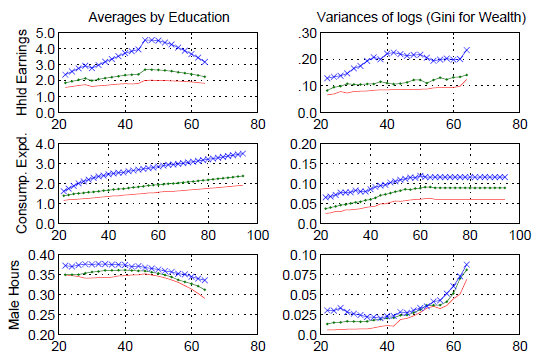
\includegraphics[width=100mm]{Figure1_1.png}\\
\tiny{Note: Statistics are presented by education. For family level variables (consumption and wealth) the education of the head (male) is used for classification. For wealth we use the absolute Gini coefficient as a measure of dispersion. Red: LH, Green: HS, Blue: CL}
\end{center}
\end{frame}


\begin{frame}[label=Life2]{Life-Cycle Profiles}
\hyperlink{Return7}{\beamerbutton{Return}}

\begin{center}
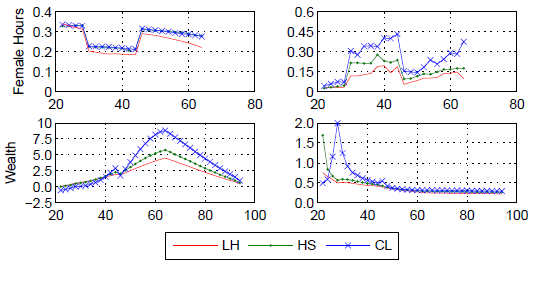
\includegraphics[width=100mm]{Figure1.png}\\
\tiny{Note: Statistics are presented by education. For family level variables (consumption and wealth) the education of the head (male) is used for classification. For wealth we use the absolute Gini coefficient as a measure of dispersion. }
\end{center}
\end{frame}


\begin{frame}[label=Extrapolate]{Extrapolating the model}
\hyperlink{Return7}{\beamerbutton{Return}}

\begin{itemize}
\item Authors extrapolated its equilibrium implications to a different time period. 
\item They set the following parameters to those prevailing
in the year 2010: (i) share parameters of different human capital in production; (ii) tuition costs and value of other education expenditures; (iii) credit limits for both subsidized and unsubsidized college loans.
\item Keeping all other parameters unchanged, authors computed a new equilibrium allocation to test how the model behaves in terms of enrollment rates and education/gender premia in 2010.
\item Very reasonable job approximating outcomes ten years out of sample.
\end{itemize}
\end{frame}

\begin{frame}[label=lstime]{Lee Seshadri sequence of events}
\hyperlink{ReturnLS1}{\beamerbutton{Return}}
\begin{center}
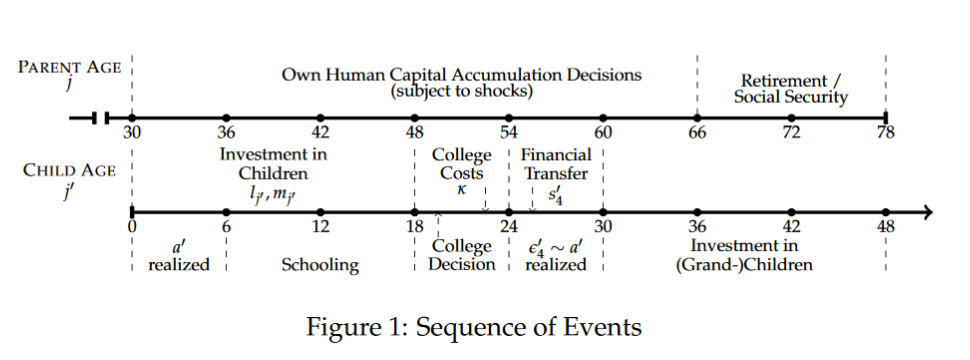
\includegraphics[width=100mm]{leeseshadri3.PNG}\\
\end{center}
\end{frame}

%%%%%%%%%%%% Discussion re Abbott paper
%% What do we want to include from these slides? These are features of the Abbott paper that we discussed on Sunday and thought were interesting. Should we cut some of this?
% \begin{frame}
% Additional discussion item slides
% \end{frame}

% \begin{frame}{Human Capital Investment}
% \begin{itemize}
% \item Model starts at age 16
% \item Estimates that much of agents income is determined by the time they make the high school completion decision (Keane and Wolpin 90\%)
% \item Heckman and Mosso (2014) discuss the literature on early childhood investments which lead to the transfer of skills from parent to child in Abbott's model but which aren't explained as tradeoffs except that the mother doesn't work full time when the child is young.
% \item Abbot et al. chose to omit the modeling of human capital development except through high school and college completion; fixing age 16 as initial conditions and also not modeling human capital investment for workers
% \end{itemize}
% \end{frame}

% \begin{frame}{Psychic costs of schooling}
% \begin{itemize}
% \item Explicitly model non-pecuniary costs of schooling as a function of gender, cognitive skills, non-cognitive skills, and a preference shock that is weighted differently for high school and college
% \item Consumption value of investment from Calcutt paper
% \end{itemize}
% \end{frame}

% \begin{frame}{Parents motivation}
% \begin{itemize}
% \item Distinction between altruism and paternalism
% \item Gender bias for altruism but not for paternalism
% \item Altruism: Parents get utility from children realizing higher future earnings (return from college)\\
% Gender specific altruism: because in the data, there's more transfers for sons than daughters? check this?
% \item Paternalism: Independent of children's outcomes, parents gain utility from child choosing to go to college\\
% Link between education - parents income is the same for sons and daughters
% This parameter $\zeta$ is fixed in the data; estimated? Ask Heckman about it? Would it affect the model?
% \end{itemize}
% \end{frame}

% \begin{frame}
% Intergenerational transmission of cog/non-cog skills between mothers and children; stuck at the bottom and top but movement in the middle of the distribution: this matches overall income mobility across generations in the literature. Should we talk about this?
% \end{frame}


% \begin{frame}{Relating Abbott to course material}
% Production function
% \begin{align*}
% Y&=F(K,\mathcal{H}) \\
% \mathcal{H}&=[s^{LH}(H^{LH})^\rho+s^{HS}(H^{HS})^\rho+s^{CL}(H^{CL})^\rho]^{1/\rho} \\
% H^e&=[s^{f,e}(H^{f,e})^\chi+s^{m,e}(H^{m,e})^\chi]^{1/\chi}
% \end{align*}
% Human capital is aggregation of 6 types of inputs: gender specific and education attainment where education takes on three categories: less than HS, HS grads and college grads. This is Katz and Murphy (1992) approach and is not in line with the skills-tasks framework we've talked about in class.
% \end{frame}

% \begin{frame}{Who makes the decision re schooling}
% \begin{itemize}
% \item In Abbott, its the child making the schooling decision conditional on transfers from parents, parents assets?, decision re borrowing,etc.
% \item Question for Professor Heckman: This is different from other intergenerational models in other papers, not sure how it matters?
% \end{itemize}
% \end{frame}

% \begin{frame}{Parent perfect info about child's skills}
% Parent has full information about childrens' skills when make the transfer decision\\
% This is a big assumption that may not be made in the other papers
% \end{frame}

% \begin{frame}{Relating Abbott to course material}
% Matching: probabilistic matching to match rates of marriage from NLSY on education dimension only//
% Simplified version of matching that we've talked about in class
% \end{frame}



% \begin{frame}
% Credit constraints: there are three sets of borrowing limits based on parent's assets; these limits seem arbitrary \\
% How are they justified? \\
% How sensitive are the results to these limits?
% \end{frame}

% \begin{frame}{Model complexity}
% Do we need to have multigenerational model? What does it add?
% Keane and Wolpin 1997 do single generation dynamic model; estimate effect of \$2000 grant for college tuition on education attainment.
% \end{frame}

\end{document}
